\clearpage
\chapter{Event Selection, Signal and Control Regions}\label{sec:selections}
We have introduced the loglead and logexclead variables, which were both highly discriminant ROI scores(Score ordering is based upon the vertex score).
Although we might have successful event selection with just triggers and ROI vertex scores, we could strengthen the discriminant power further if we consider objects other than the trigger and ROIs(tracks).
These variables could be
\begin{itemize}
 \item Non-relevant to ROIs (muon, jet object)
 \item Missing input variable in the ROI training
\end{itemize}
These are not ML training inputs; something ML cannot learn.
So they are not discriminated against with scoring of the ROIs.
The analysis implements other event selection categories itemized below for this phenomenological situation.
\begin{itemize}
  \item $\Delta\Phi(lead ROI,sublead ROI)$ 
  \item $\Delta R(lead ROI, Jet)<$0.6 
  \item 1 Isolated $\mu$
  \item Leading $\mu$'s transverse impact parameter significance to PV
\end{itemize}

Each of the cuts for the items above is motivated and explained in following subsections.

\section{Isolation criteria for muons}\label{ref:muISO}
As discussed in ~\ref{sec:triggers}, the main background for our analysis comes from QCD process, especially from the B-meson decay of QCD events with high ROI scores.
Leptonic decay of B-meson generates muons, which trigger the B-parking trigger of the analysis.
Muons of B-meson decay have inferior isolation quality.
They come with other hadron tracks near themselves in B-meson decay process.
In contrast, muons of $\tau$ lepton decay have better isolation quality.
As shown in the figure \ref{fig:tdet}, $\tau$ lepton has no hadron decay associated with muon when it decays into a muon.
In order to eliminate the dominant B-meson background from the QCD process, the analysis applies a PFISOLoose in selecting muon objects.
The precise definition of PFISOLoose is defined below.
\begin{itemize}
  \item $(\Sigma pT(ch.had from PV)+max(0,\Sigma ET(neut.had) \Sigma ET (phot)-0.5* \Sigma pT(ch.had from PU)))/P_{T}(\mu)<0.25$
\end{itemize}

%Not only muons decayed from $\tau$ leptons with 55, 40GeV mass have a good isolation quality, but also muons of $\tau$ leptons from 15 GeV have a decent isolation quality based on gen-level $\Delta R(\tau,\bar_{\tau})$.
Due to its poorer isolation quality from the boost, some muons decayed from $\tau$ lepton with a 7\GeV mass fail isolation cut.
However, applying the PFISOLoose cut on muons is still beneficial since it removes more background events than signal events.
The table below demonstrates event yield drop before and after requiring PFISOLoose cut on muons, classified by its signal and background process.


\begin{tiny}
    \begin{table}
  \centering
\begin{tabular}{|p{3cm}|p{2cm}|p{2cm}|}
\hline
MC sample & events with BPH+1$\mu$ (noISO) & events with BPH+1$\mu$ (ISO) \\
\hline
 15to20 & 1 & 0.545 \\
 \hline
 20to30 & 1 & 0.407 \\
\hline
 30to50 & 1 & 0.295 \\
\hline
 50to80 & 1 & 0.144 \\
\hline
 80to120 & 1 & 0.078 \\
\hline
120to170 & 1 & 0.049 \\
\hline
170to300 & 1 & 0.032 \\
\hline
\textcolor{red}{ggH4$\tau$-MS7}& 1 & 0.619 \\
\hline
\textcolor{red}{ggH4$\tau$-MS15} & 1 & 0.855 \\
\hline
\textcolor{red}{ggH4$\tau$-MS40} & 1 & 0.910 \\
 \hline
    \end{tabular}
    \caption{Ptbinned Isocut}
    \end{table}
\end{tiny}    

One can also gauge the isolation of muon object based on the generator level of $\Delta$R of tau lepton pair as in figure \ref{fig:taudeltaR}.
 \begin{figure}[h!]
   \caption{$\Delta$R value of tau lepton pair from LLP decay is plotted. $\tau$s' mass are low enough to be resolved when decayed from heavier LLP.}
   \label{fig:taudeltaR}
   \centering
   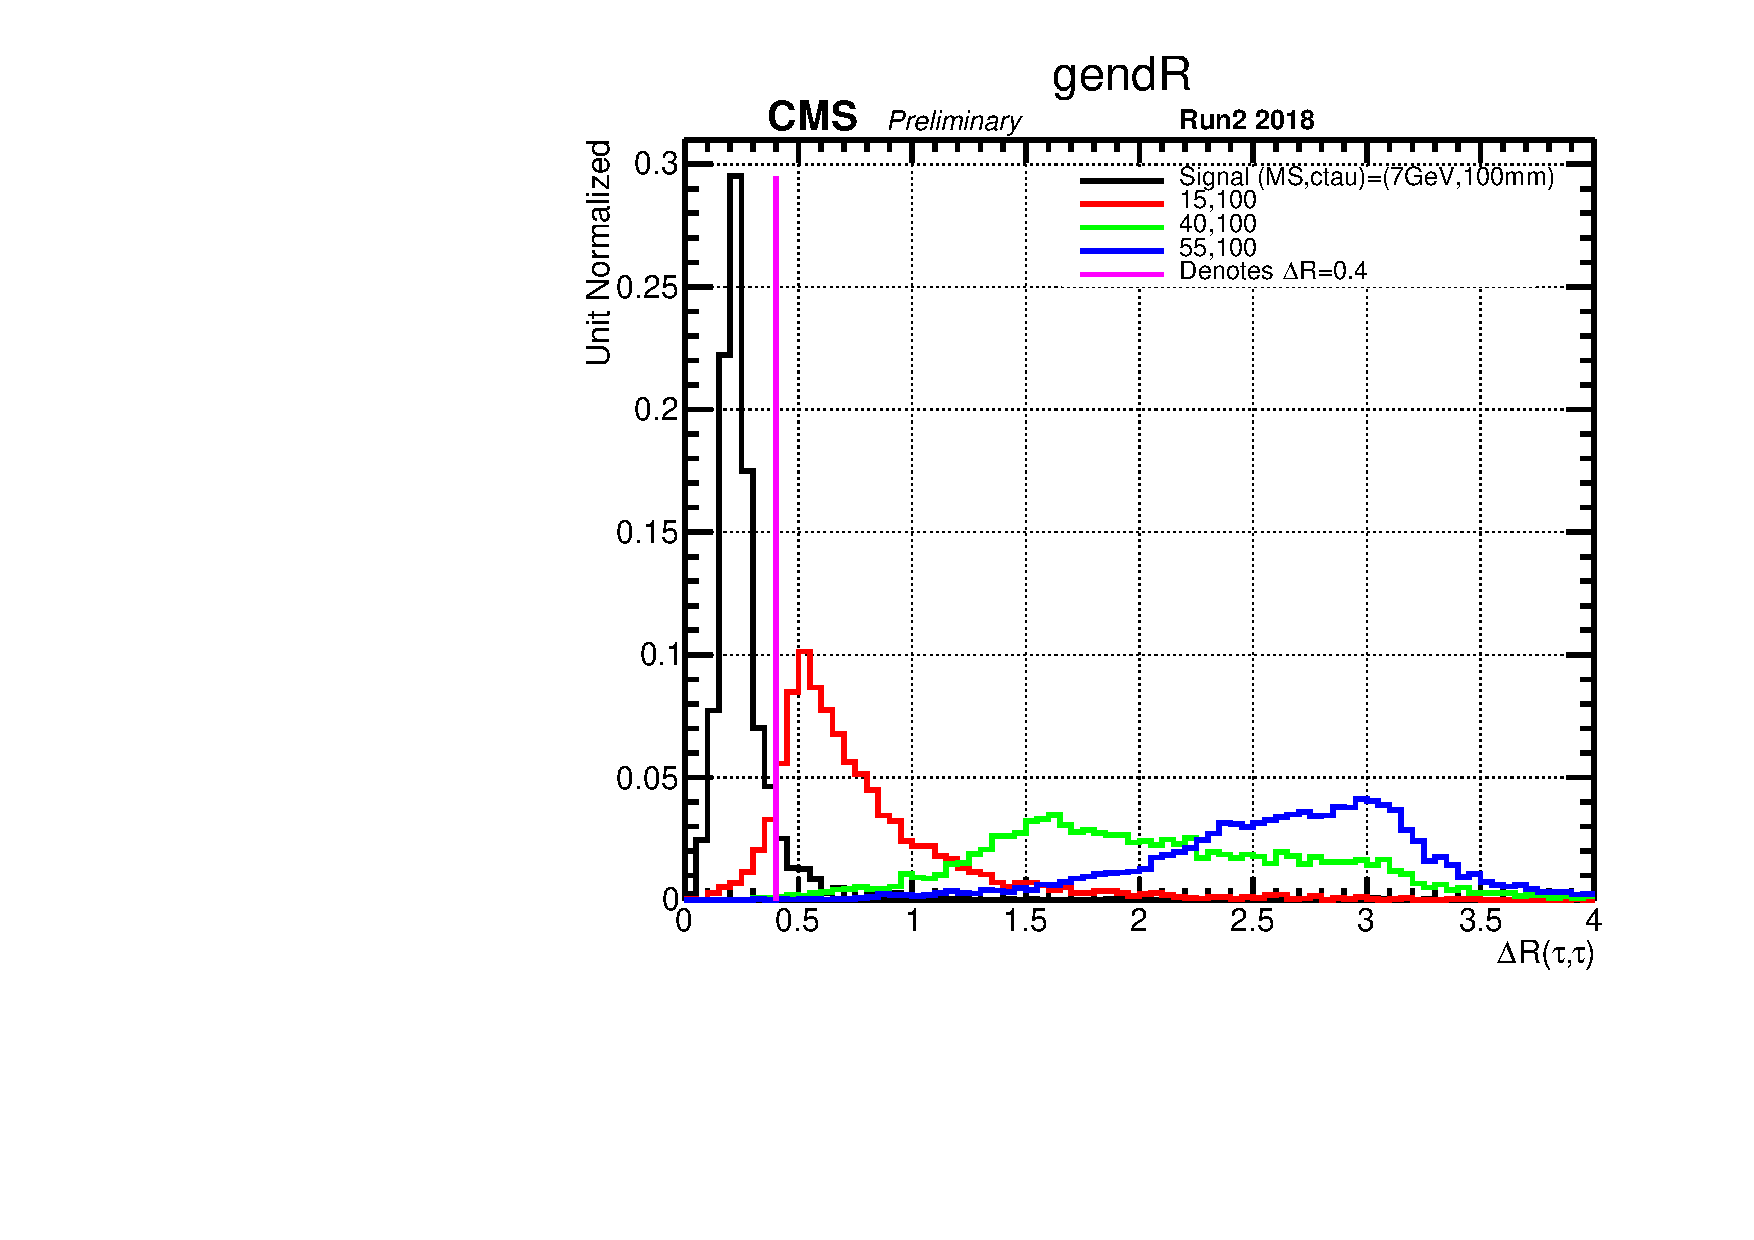
\includegraphics[width=0.60\linewidth]{figs/taugendR.pdf}
 \end{figure}





\section{Delta Phi(lead ROI,sublead ROI)}\label{sec:DeltaPhi}
This analysis looks for displaced vertices in the tracker region, coming from the decays of exotic LLPs from Higgs produced in gluon fusion mode, leaving the SM Higgs boson without boost.
The largest mass of the exotic LLPs is 55\GeV, ranging down to 7\GeV.
Thus, exotic LLPs decayed from the SM Higgs become boosted, with their momentum vectors pointing back-to-back in the SM Higgs rest frame.
Exotic LLPs with lighter mass are more boosted than heavier LLPs since less LLP mass means more leftover energy into kinetic energy.
Given that ROIs corresponding to an exotic LLP's decay should have the highest ROI score, one should expect that the leading ROI and subleading ROI in a single event would be back-to-back.
Thus, in signal events, $\Delta\Phi$(lead ROI,sublead ROI) tends to have high values, while the background processes tend to have a more random distribution.
This analysis applies a cut above 2.2 to reduce background contribution.

%Figure ~\ref{fig:dPhileadsub} shows the difference between the distribution of signal process and SM QCD backgrounds.


 \begin{figure}[h!]
   \caption{Signal versus Background for Delta Phi(leadROI, subleadROI). Left plot is for MS-15\_ctauS-10mm point, whereas the right plot is for MS-15\_cauS-100mm point}
   \label{fig:leadexcPosPhi}
   \centering
   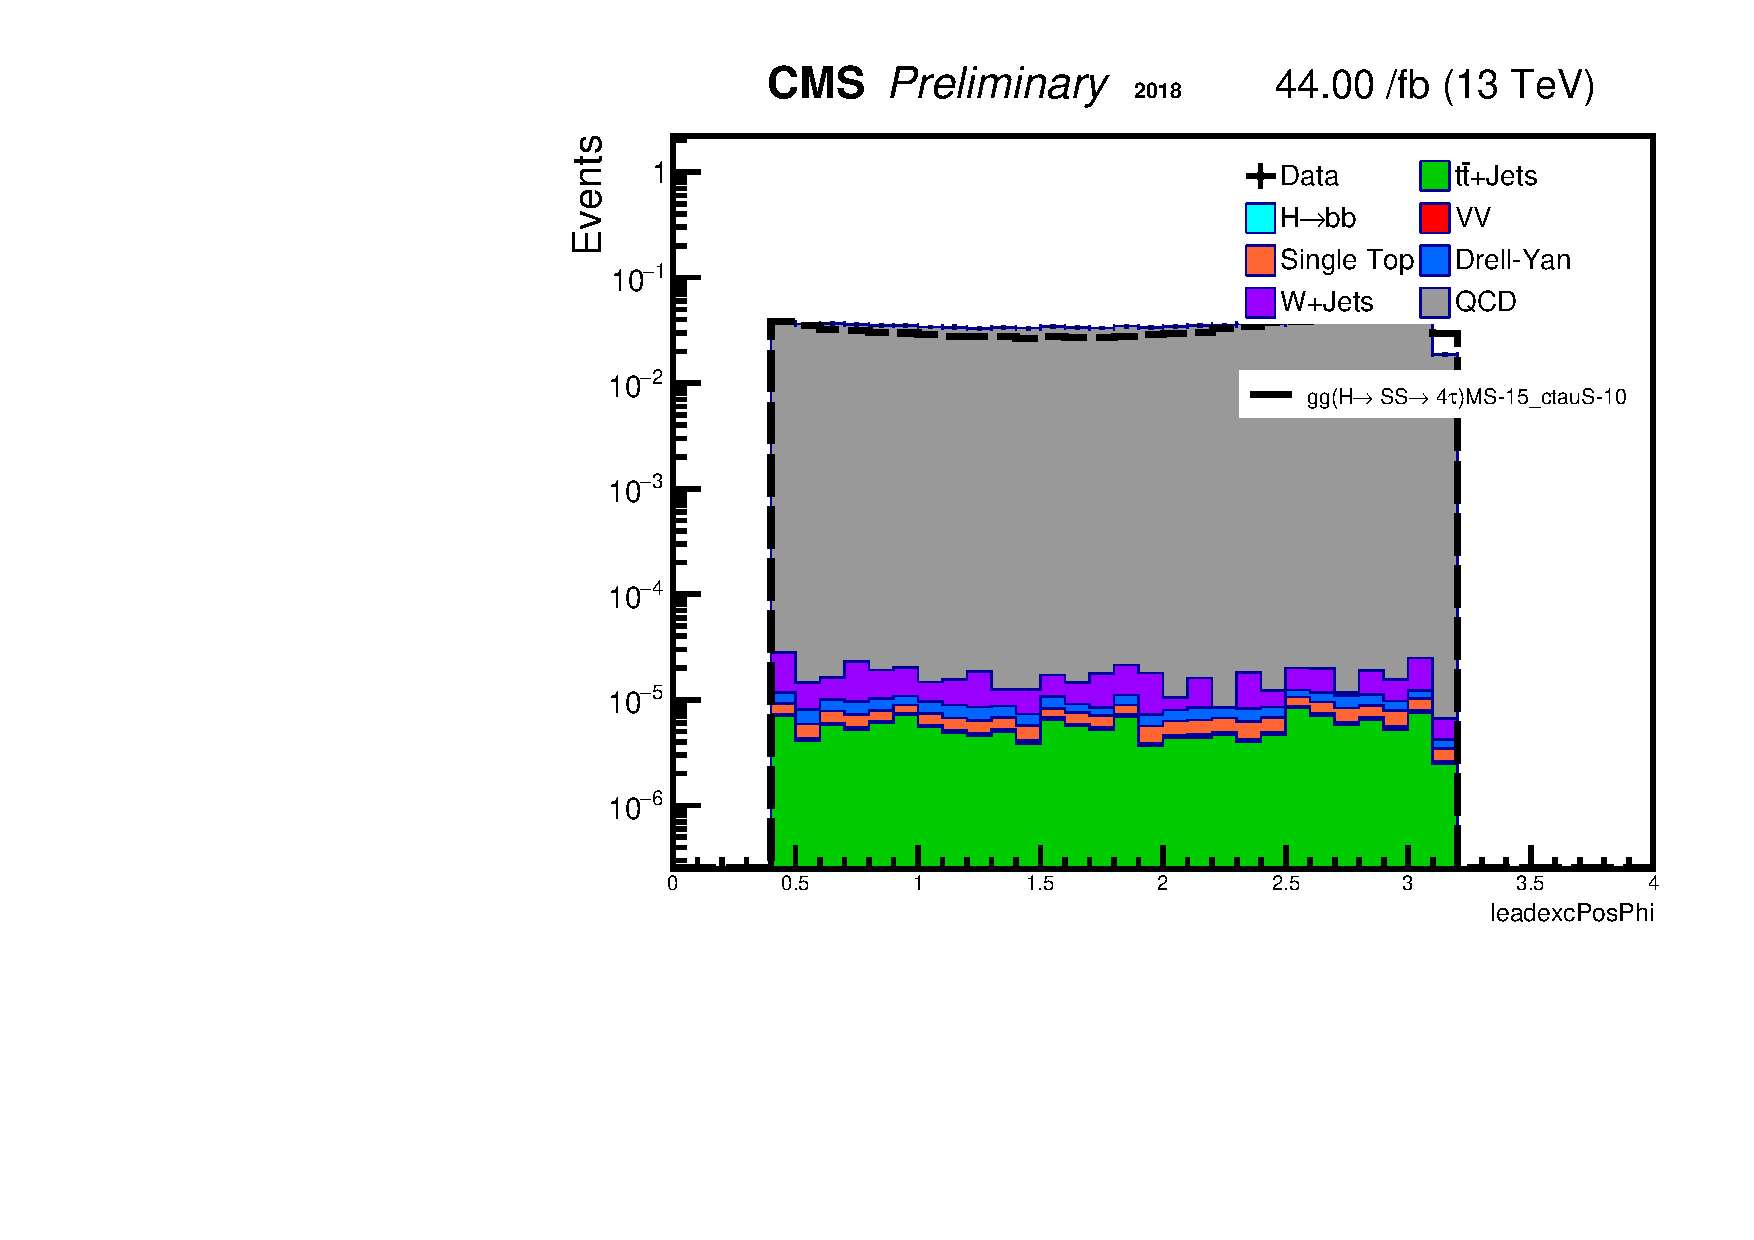
\includegraphics[width=0.40\linewidth]{figs/log_Oct6ANVars_MS-15_ctauS-10_leadexcPosPhi.pdf}
   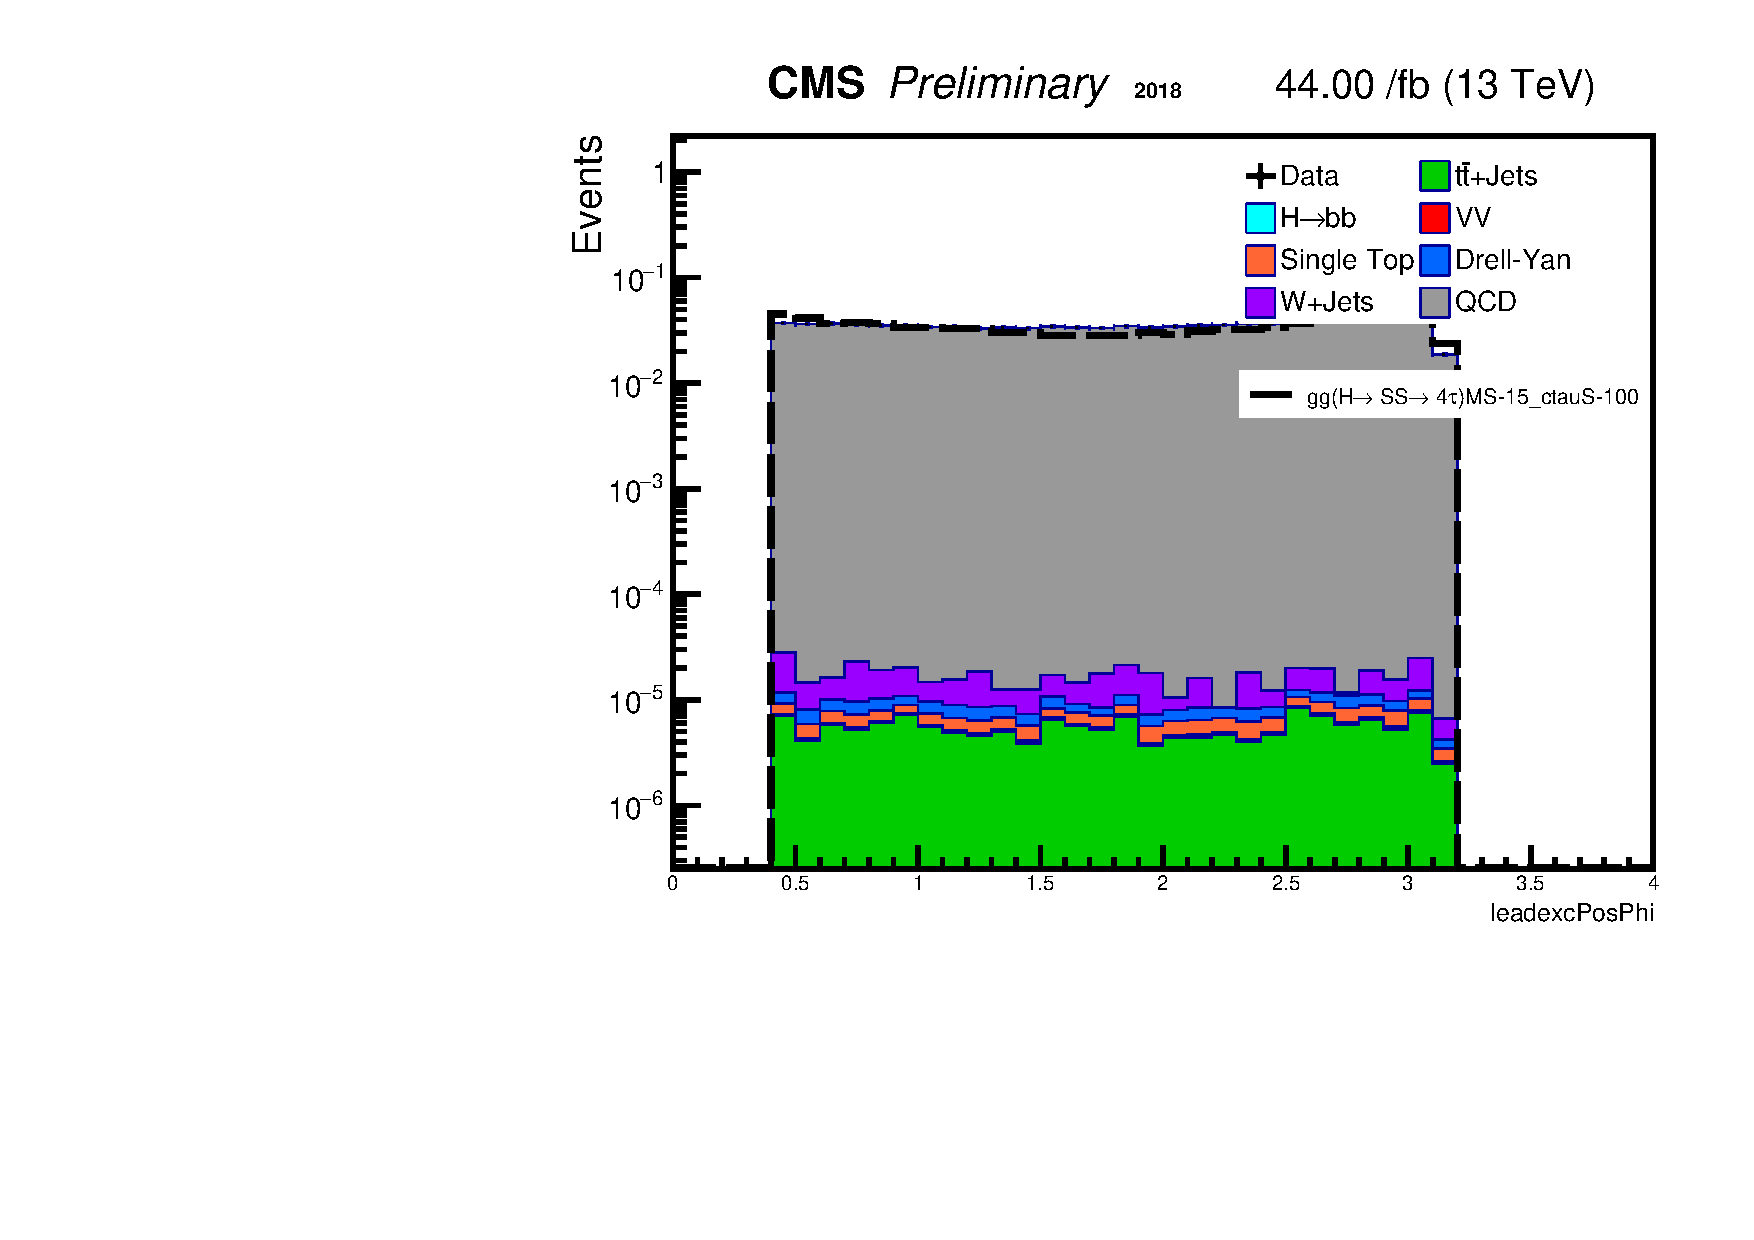
\includegraphics[width=0.40\linewidth]{figs/log_Oct6ANVars_MS-15_ctauS-100_leadexcPosPhi.pdf}
 \end{figure}


\section{DeltaR(ROI, jet)}\label{ref:jetdR}
$\tau$ leptons of the signal process can also decay hadronically, while only one of the $\tau$ leptons decay into a muon to trigger the B parking trigger.
When $\tau$ leptons decay, its decay shower can get clustered in the calorimeter and reconstructed as a jet.
Given that the $\tau$ lepton's on-shell mass is a fixed value, $\tau$ lepton and its hadronic decay products (to be clustered into a jet) have a specific kinematic phase space.
Thus, the $\Delta$ R(ROI, jet) has a distribution with a peak at a value around 0.3-0.6.
Meanwhile, the QCD background has a different distribution shape.
Given the hadronic nature of the process, jet multiplicity is high.
Higher jet multiplicity makes the $\Delta$ R(ROI, jet) value somewhat randomized, resulting in a flat distribution.


 \begin{figure}[h!]
   \caption{Delta R(Jet, leadingROI). Left plot is for MS-15\_ctauS-10mm point, whereas the right plot is for MS-15\_cauS-100mm point}
   \label{fig:JetDeltaRleadSize}
   \centering
   \includegraphics[width=0.47\linewidth]{figs/log_Oct6ANVars_MS-15_ctauS-10_leadcloseJetdR.pdf}
   \includegraphics[width=0.47\linewidth]{figs/log_Oct6ANVars_MS-15_ctauS-100_leadcloseJetdR.pdf}
   \includegraphics[width=0.47\linewidth]{figs/log_Oct6ANVars_MS-15_ctauS-1000_leadcloseJetdR.pdf}
   \includegraphics[width=0.47\linewidth]{figs/log_Oct6ANVars_MS-55_ctauS-10_leadcloseJetdR.pdf}
 \end{figure}

\section{Leading muon's transverse impact parameter significance to PV}\label{ref:muIP}

With the B-Parking trigger, triggering muons have significant transverse displacement (impact parameter) in both background and signal processes.
However, displacement in the signal process is more significant than in the background process.
The signal process has a minimum of c$\tau$ = 1mm, which is longer than the B-meson lifetime.
Thus, triggering muon object's transverse impact parameter to PV (muIPSig) is larger in the signal process than in the background process.
In order to account for the error values associated with the parameter, we use impact parameter significance, defined as the ratio of the impact parameter divided by its error.
In order to adjust the orders of the magnitude observed for the impact parameter significance (muIPSig) variable, we exploit the log value of the IPSig.
The analysis implements a cut on Log10(muIPSig).


 \begin{figure}[h!]
   \caption{leading muon's transverse impact parameter value to the primary vertex. Left plot is for MS-15\_ctauS-10mm point, whereas the right plot is for MS-15\_cauS-100mm point}
   \label{fig:leadmuIP}
   \centering
   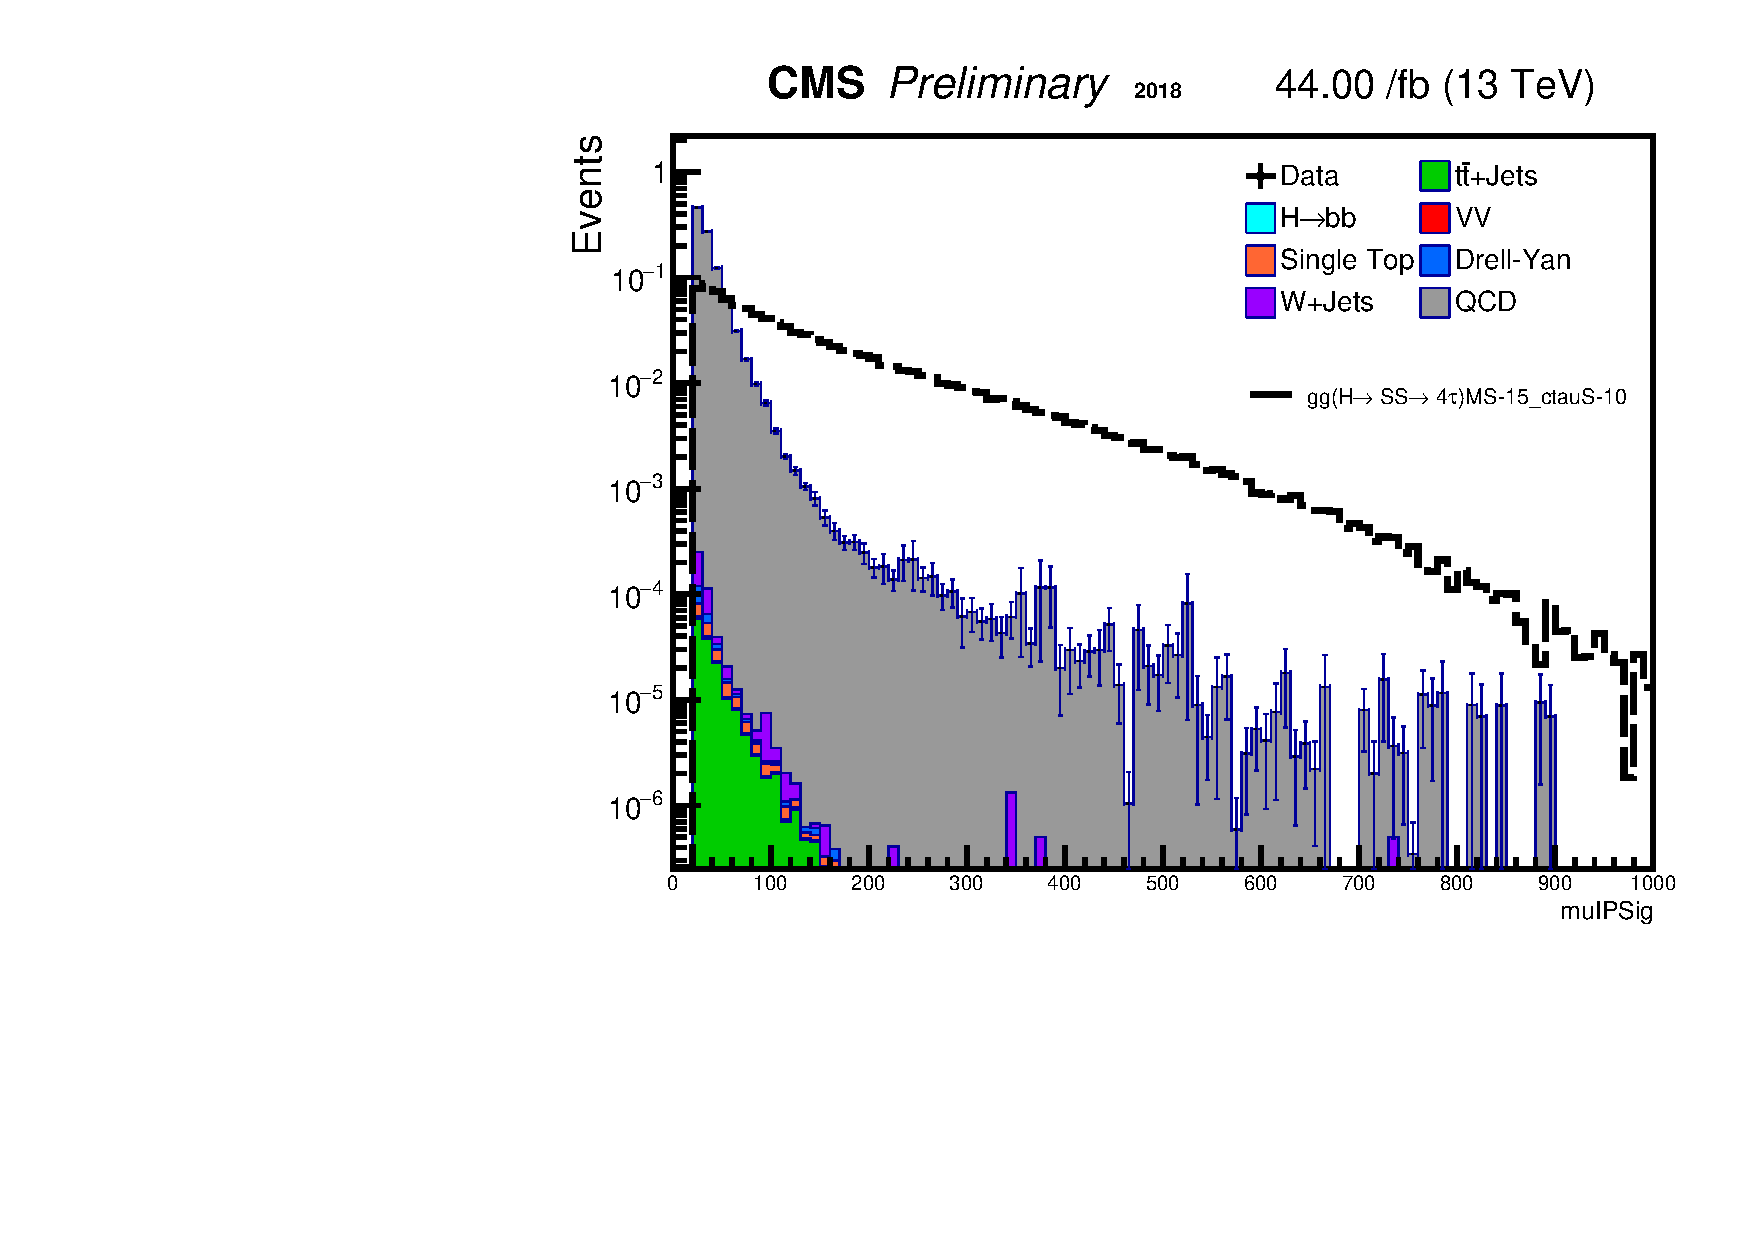
\includegraphics[width=0.47\linewidth]{figs/log_Oct6ANVars_MS-15_ctauS-10_muIPSig.pdf}
   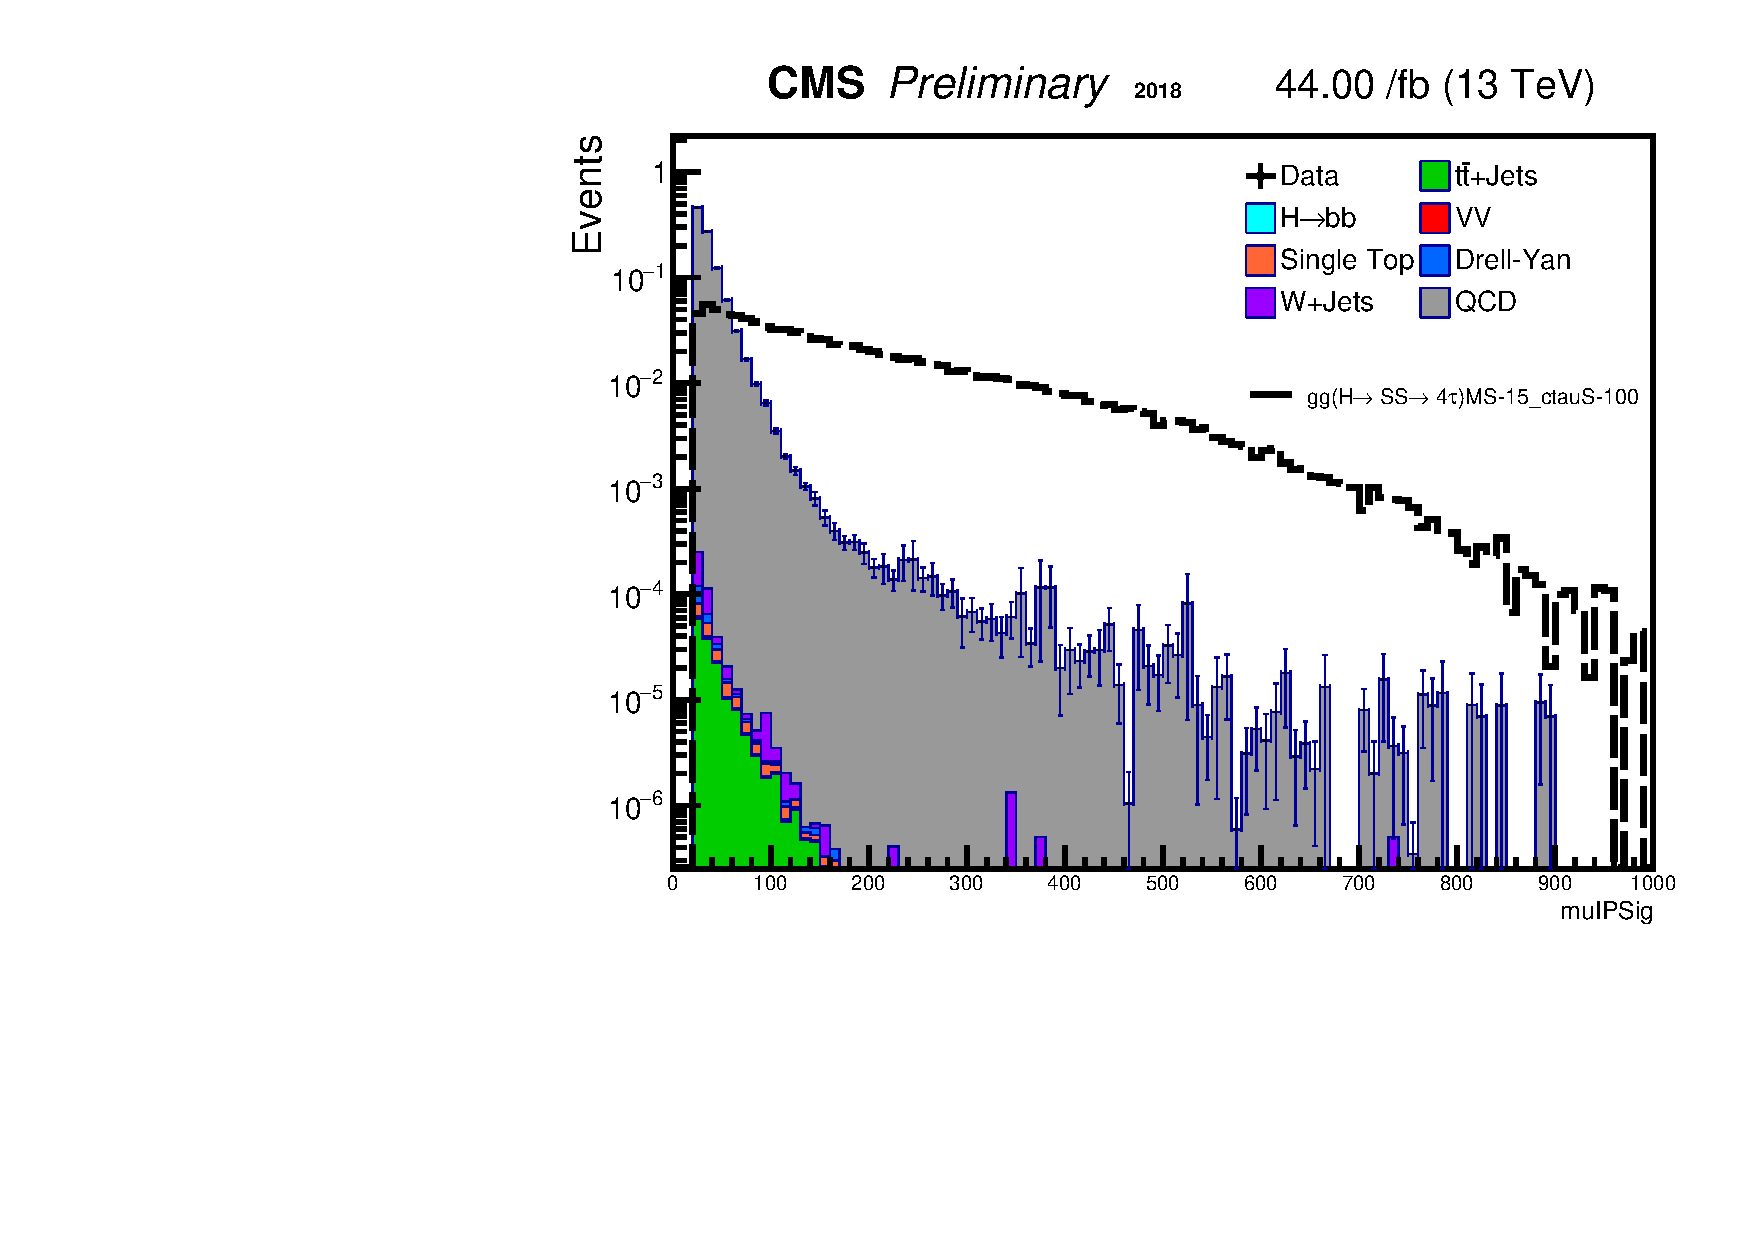
\includegraphics[width=0.47\linewidth]{figs/log_Oct6ANVars_MS-15_ctauS-100_muIPSig.pdf}
   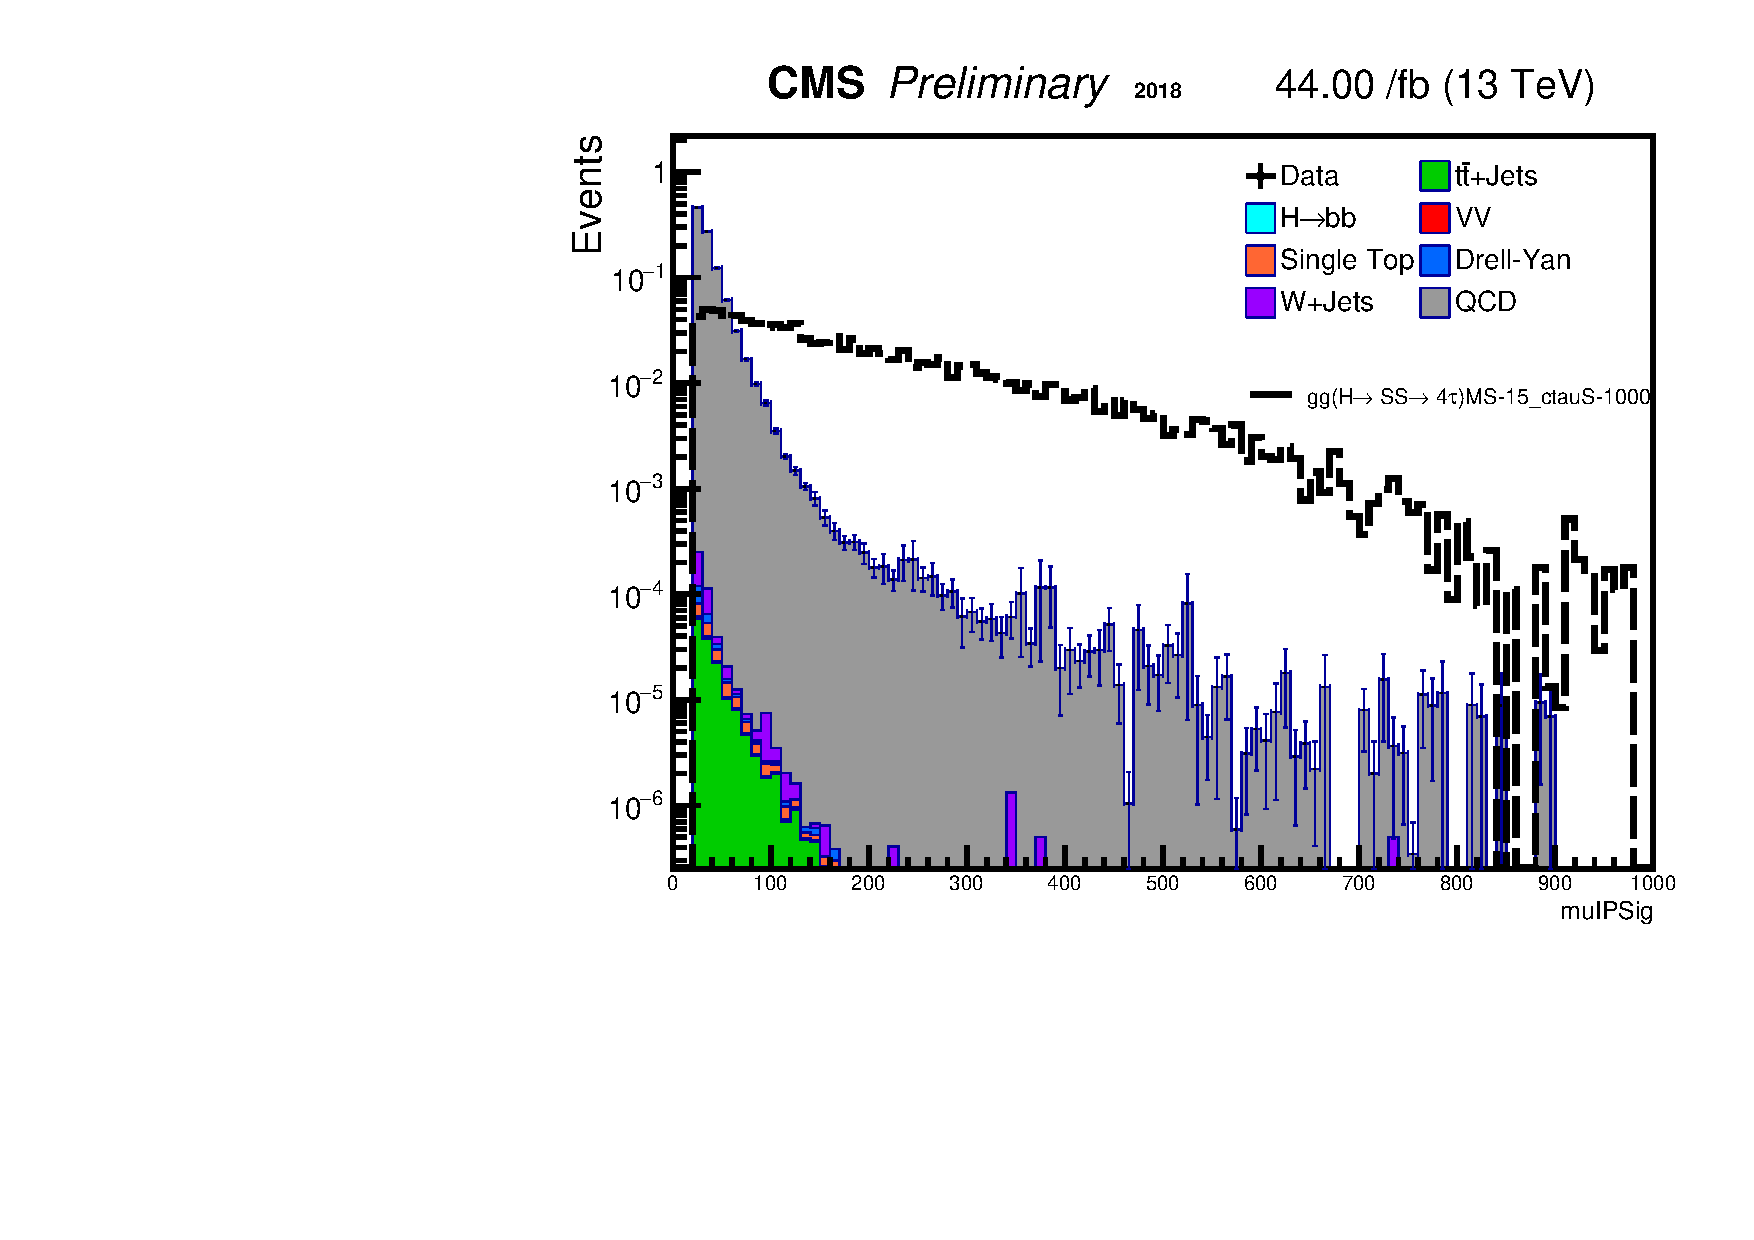
\includegraphics[width=0.47\linewidth]{figs/log_Oct6ANVars_MS-15_ctauS-1000_muIPSig.pdf}
   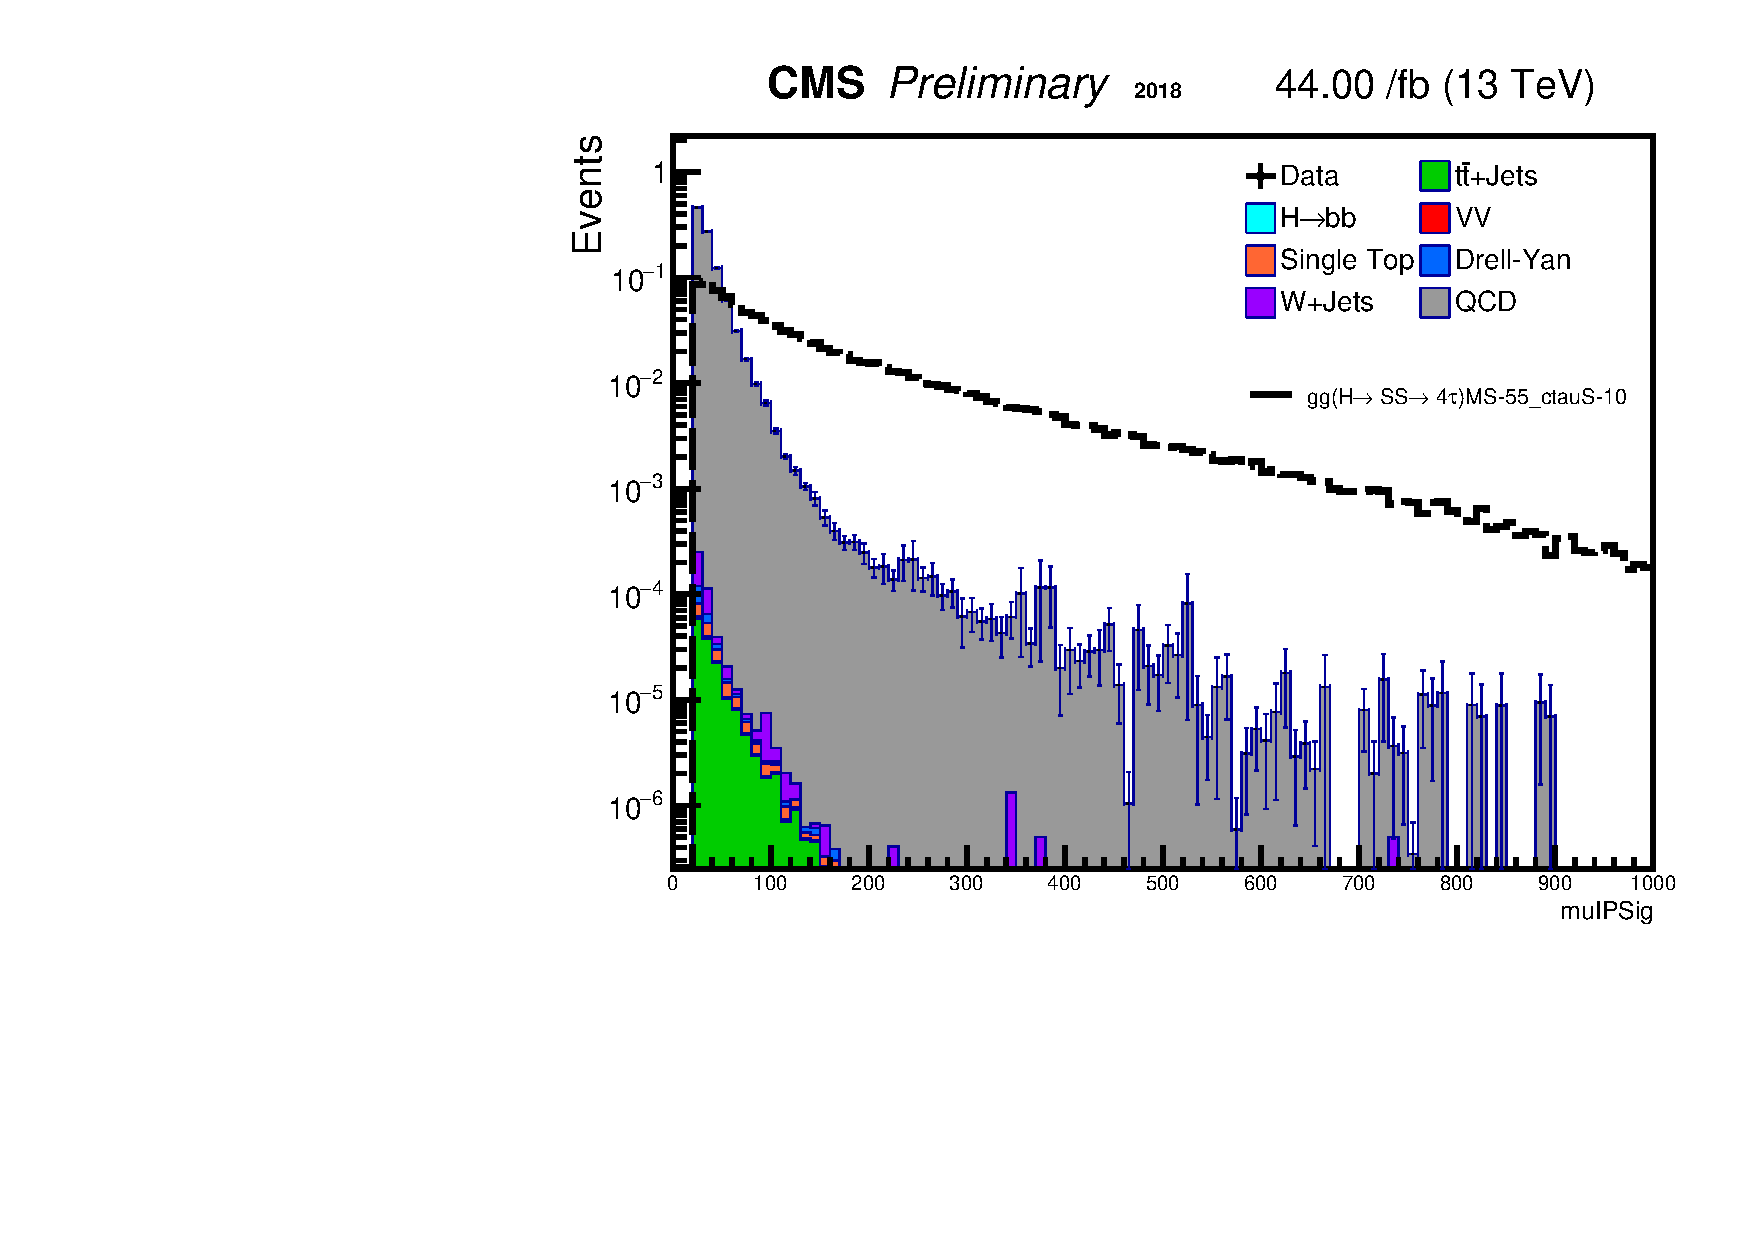
\includegraphics[width=0.47\linewidth]{figs/log_Oct6ANVars_MS-55_ctauS-10_muIPSig.pdf}
 \end{figure}

 \begin{figure}[h!]
   \caption{Amplified histograms of Log10muIPSig}
   \label{fig:AmpleadmuIP}
   \centering
   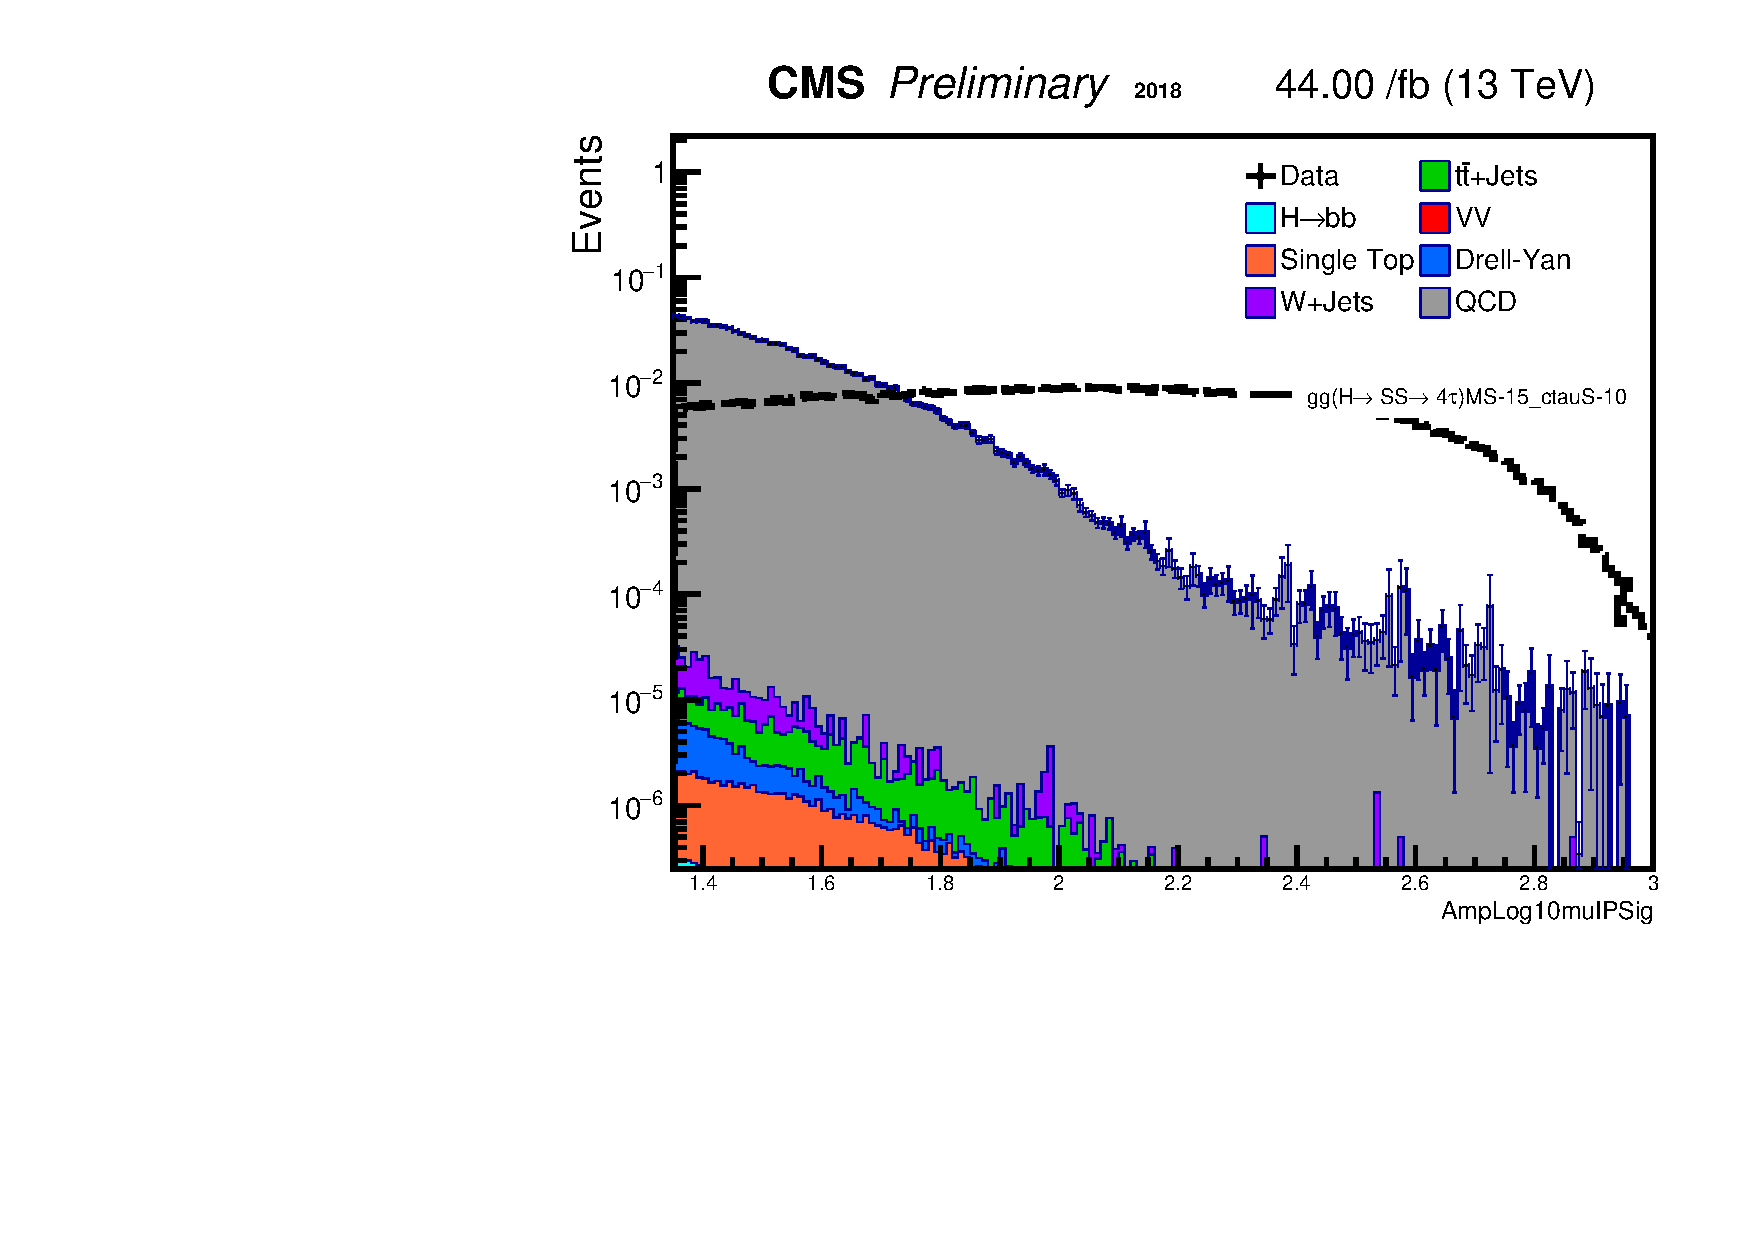
\includegraphics[width=0.47\linewidth]{figs/log_Oct6ANVars_MS-15_ctauS-10_AmpLog10muIPSig.pdf}
   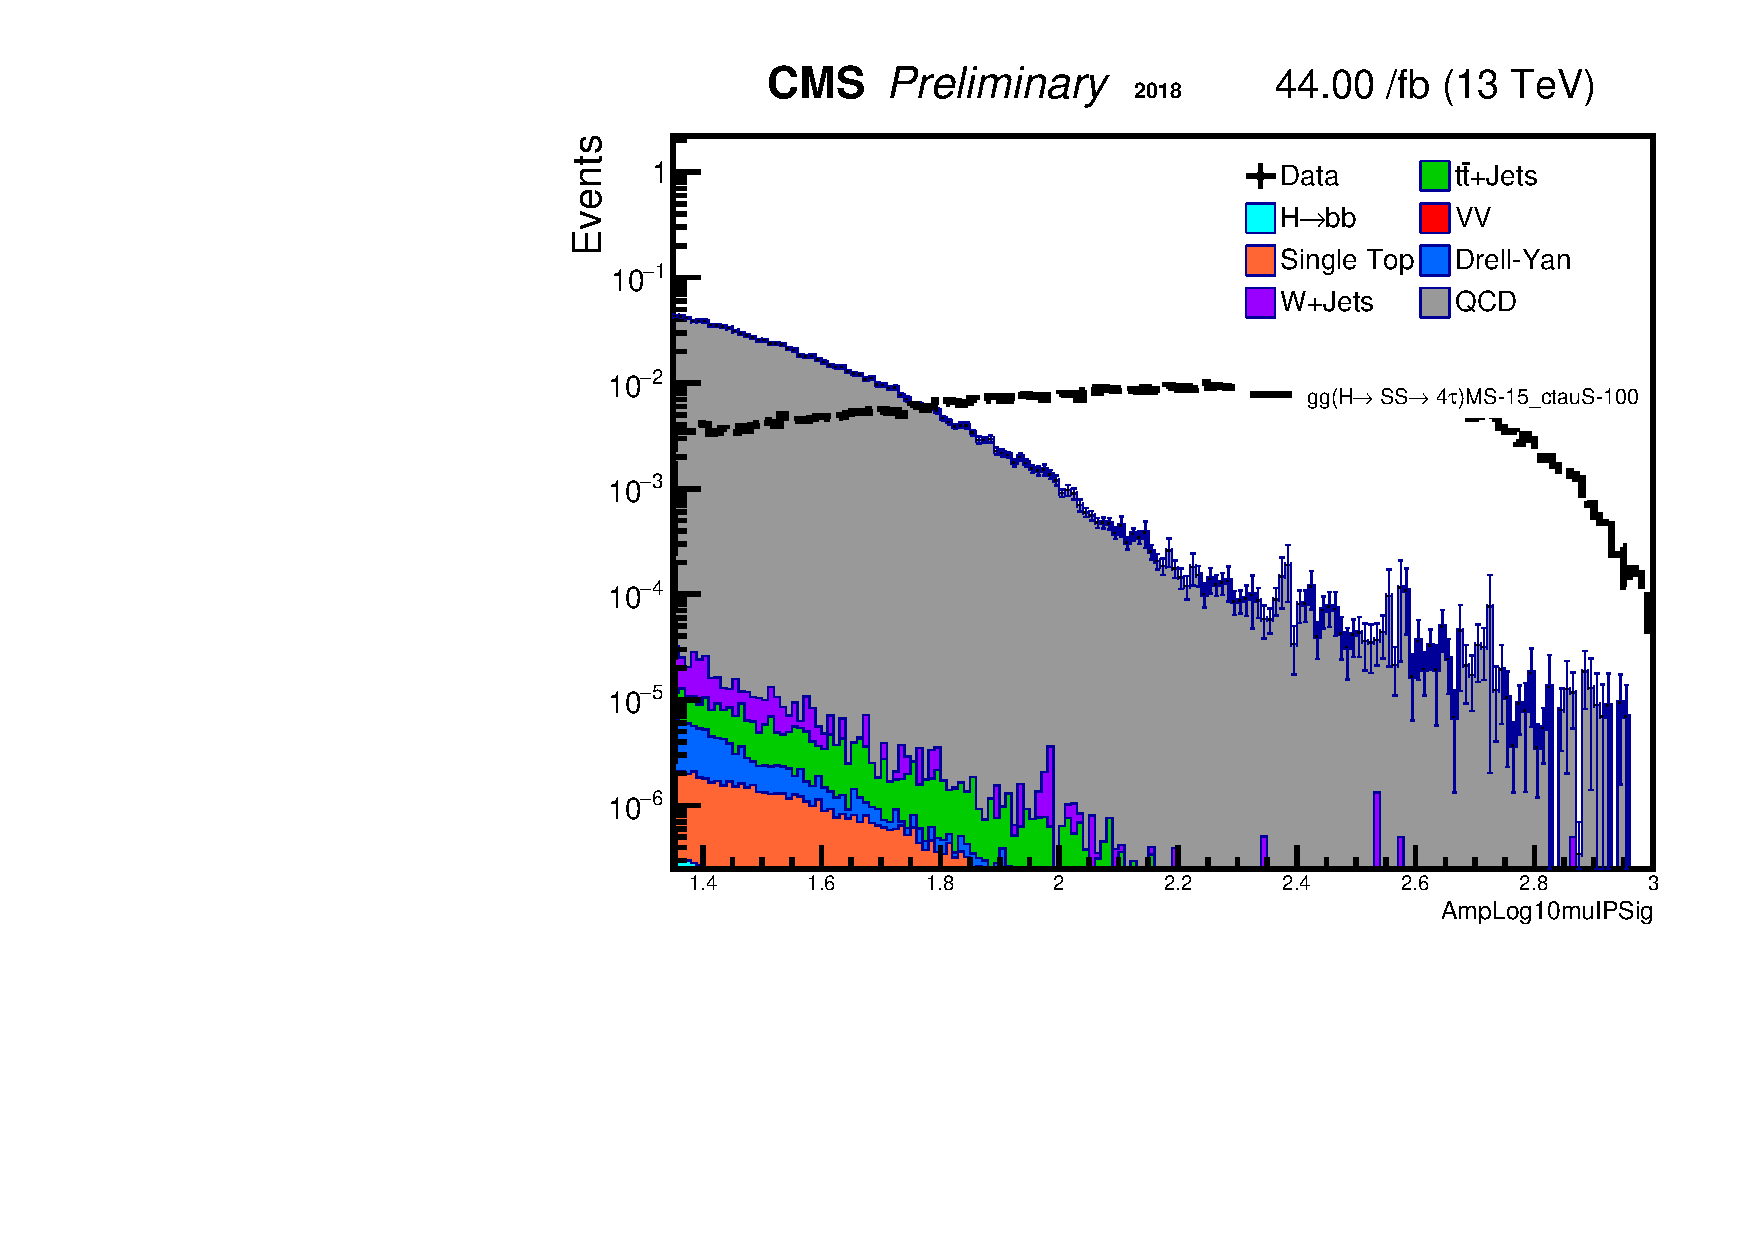
\includegraphics[width=0.47\linewidth]{figs/log_Oct6ANVars_MS-15_ctauS-100_AmpLog10muIPSig.pdf}
   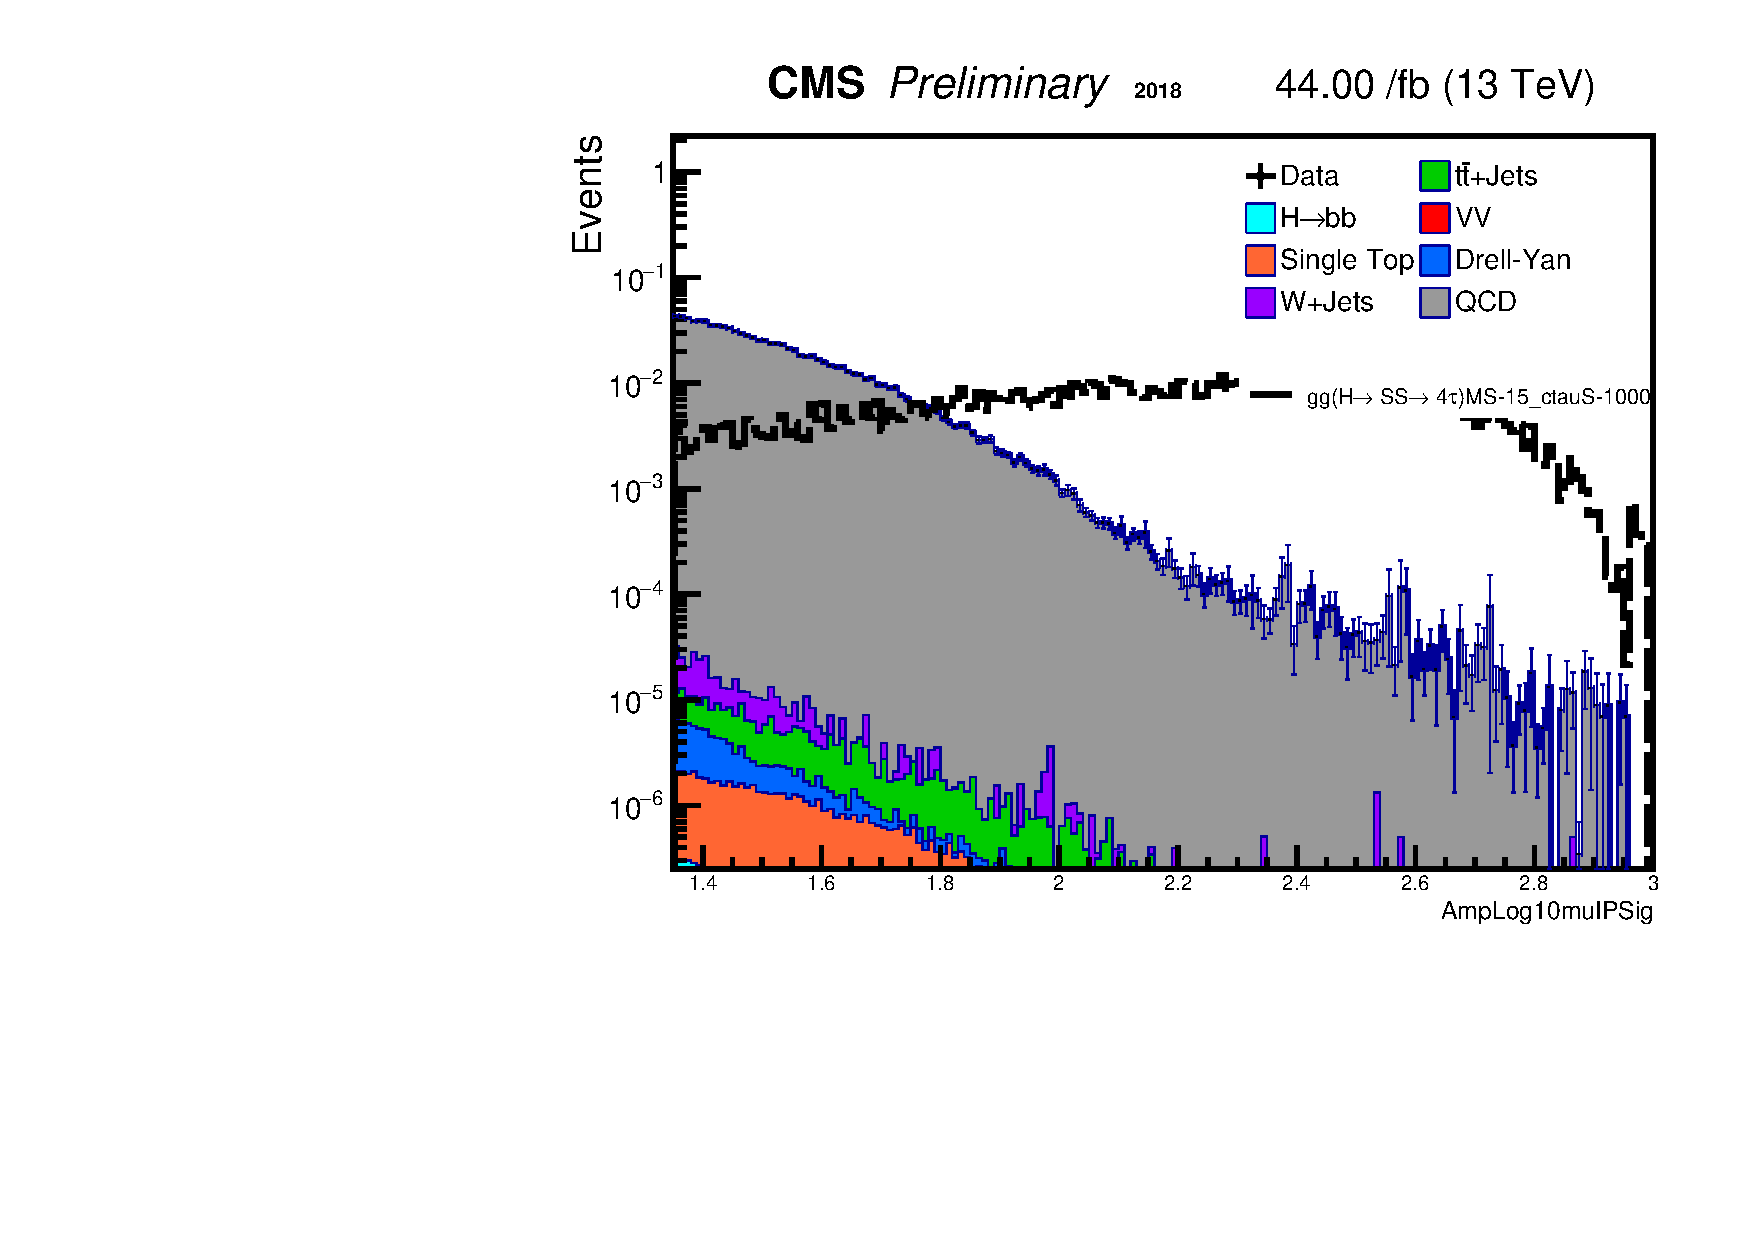
\includegraphics[width=0.47\linewidth]{figs/log_Oct6ANVars_MS-15_ctauS-1000_AmpLog10muIPSig.pdf}
   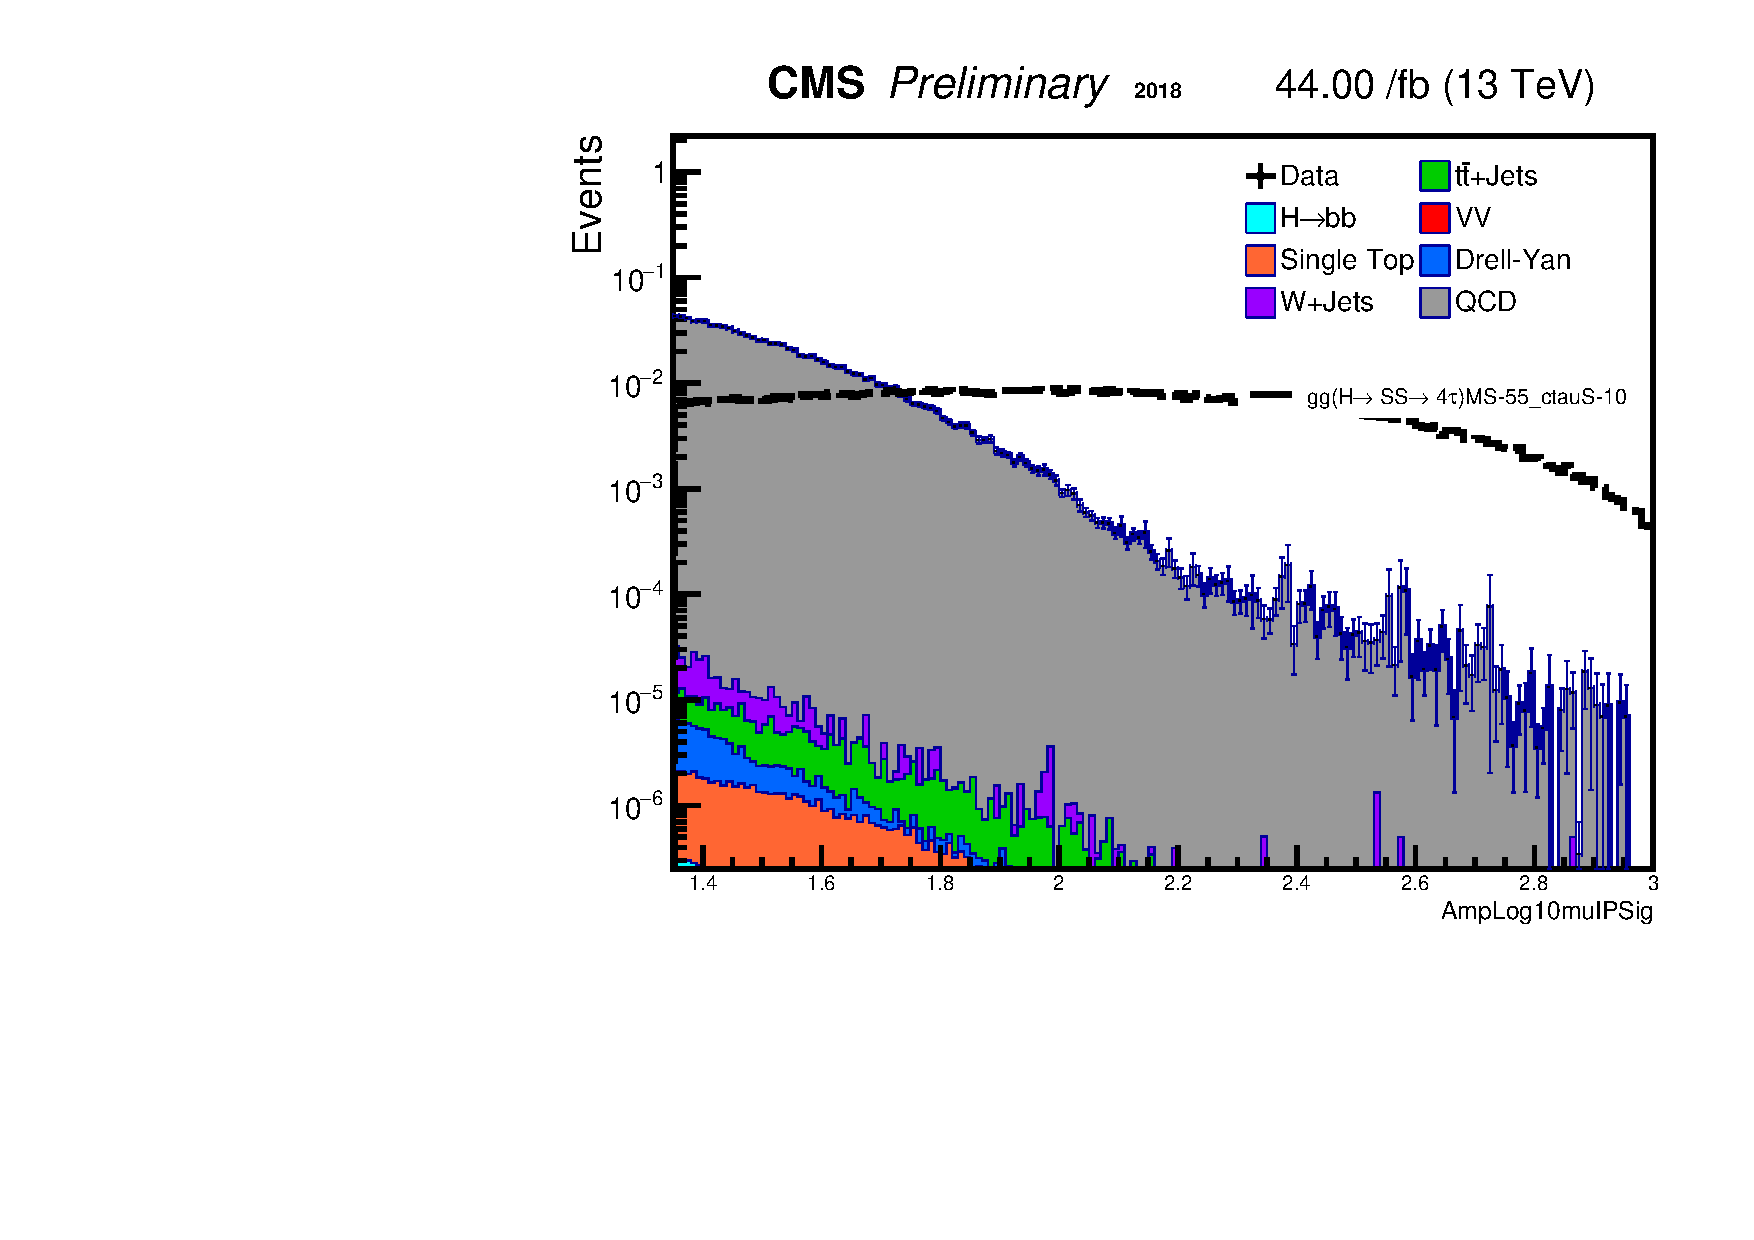
\includegraphics[width=0.47\linewidth]{figs/log_Oct6ANVars_MS-55_ctauS-10_AmpLog10muIPSig.pdf}
 \end{figure}

\begin{figure}[h!]
  \caption{Data/MC agreement for distributions}
  \label{fig:DataMCscore5}
  \centering
  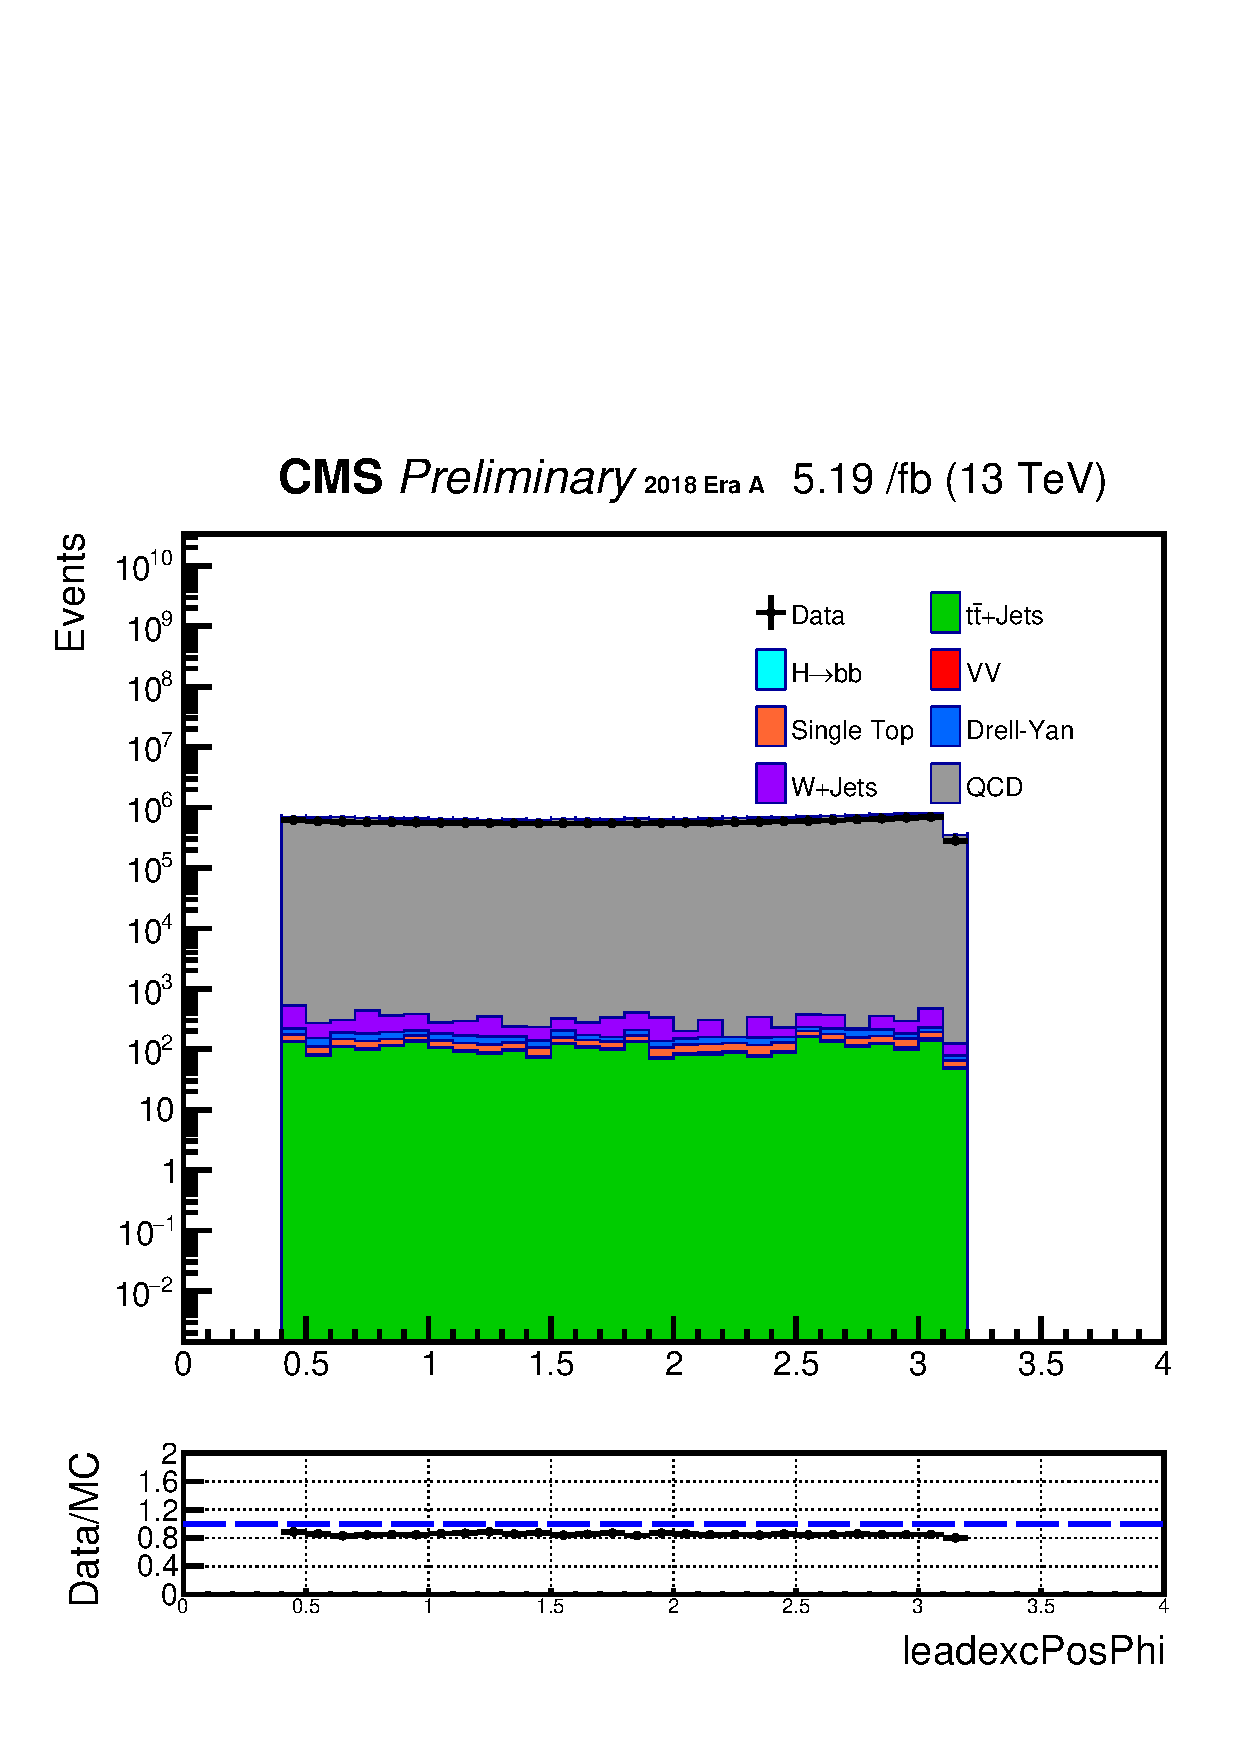
\includegraphics[width=0.40\linewidth]{figs/Data_log_Oct6ANVars_MS-15_ctauS-10_leadexcPosPhi.pdf}
  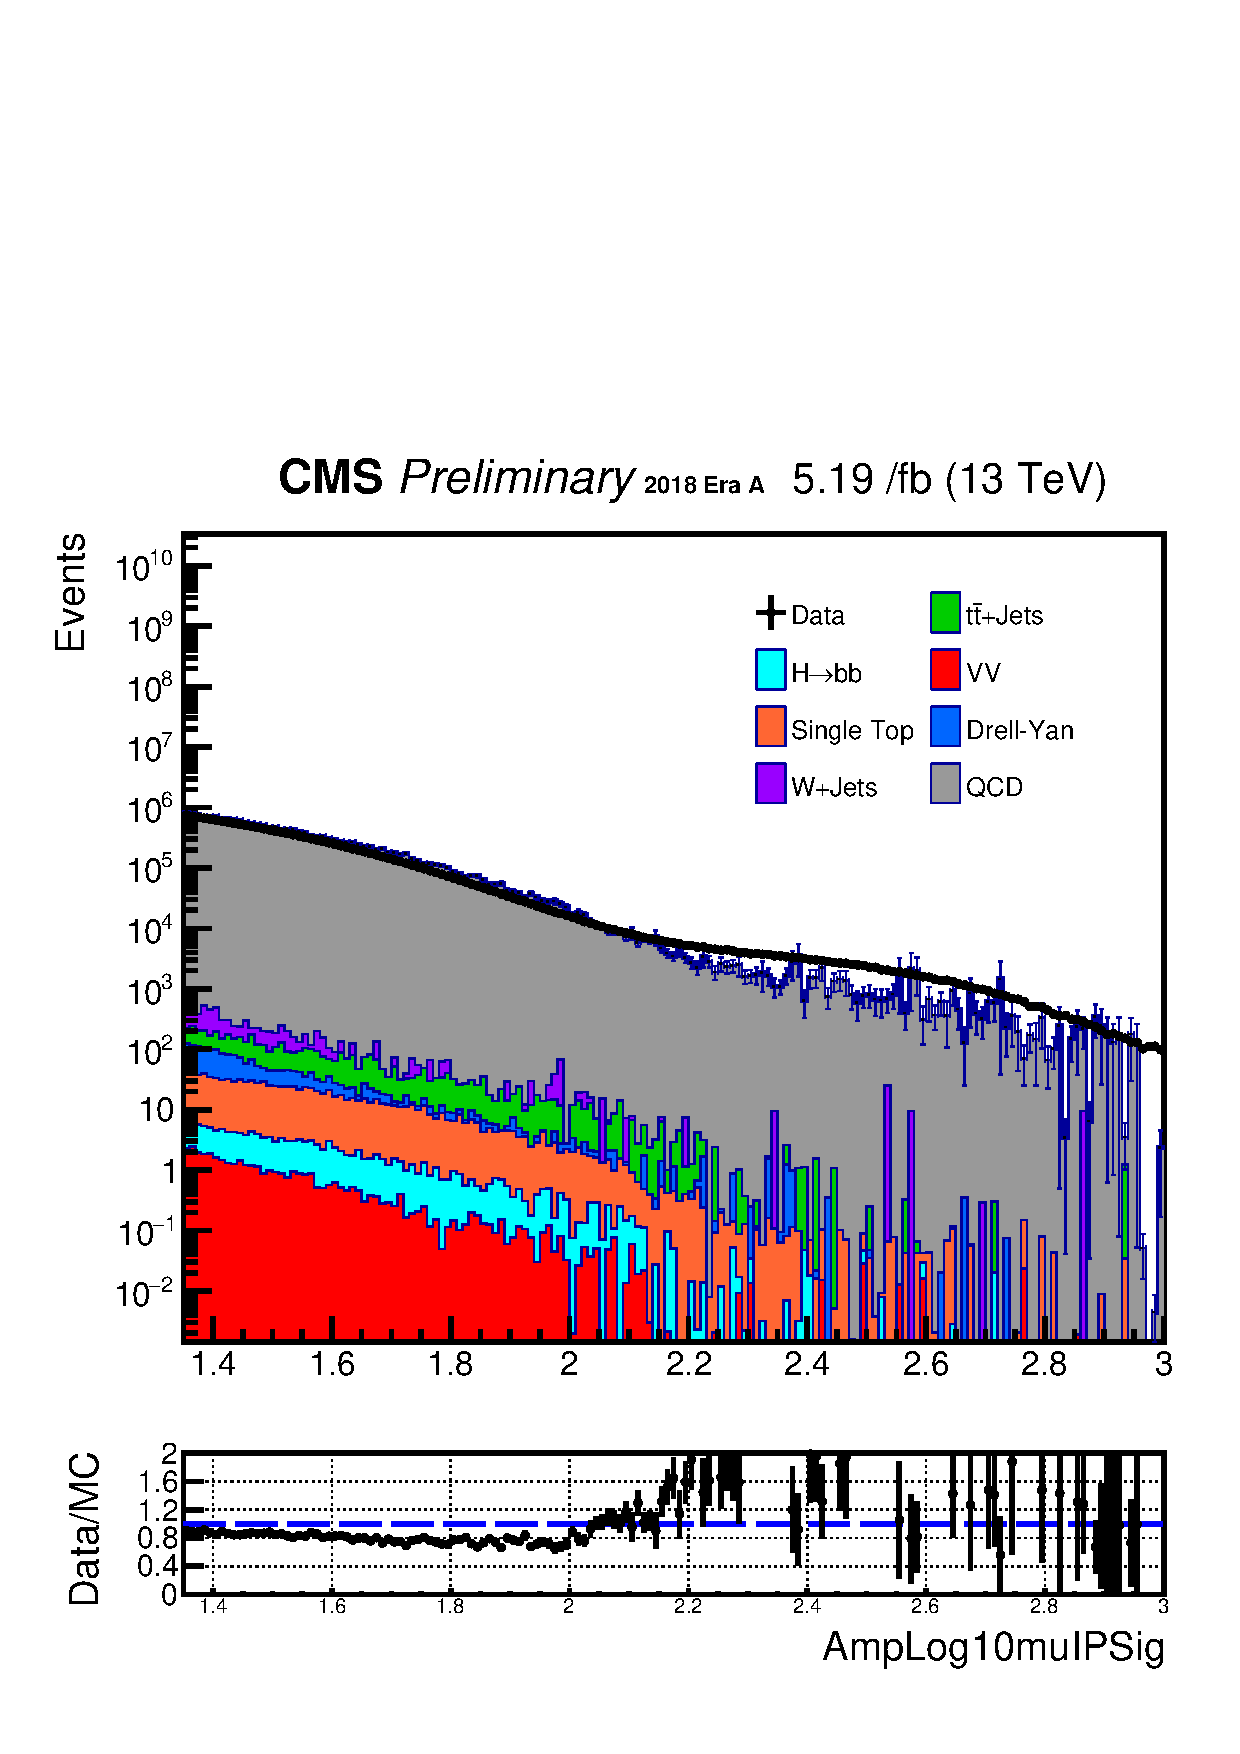
\includegraphics[width=0.40\linewidth]{figs/Data_log_Oct6ANVars_MS-15_ctauS-10_AmpLog10muIPSig.pdf}
  \includegraphics[width=0.40\linewidth]{figs/Data_log_Oct6ANVars_MS-15_ctauS-10_leadcloseJetdR.pdf}

\end{figure}

%\section{Number of Annulus Tracks Associated with ROI}
% The tensorflow used for this analysis is trained with $p_T, \eta, \chi^{2}$, and other information of the annulus tracks (tracks that are inside ROI radius, but not fitted to vertex).
%Meanwhile, an ROI's total number of annulus tracks is not a direct input for ML and tensorflow can only learn such information indirectly via annulus tracks' $p_T$.
%Although having selected ROIs with high scores ($>$0.999), signal processes ROIs' number of annulus tracks show a quite different distribution from the background process.
%%Figure ~\ref{fig:ANnum}
%signal's high-scoring ROIs are mostly from the the exotic LLP scalar's decay into $\tau$ leptons. 
%%The $\tau$ leptons have most 3 charged tracks for 12\%, and 1 charged track for 80\% of its decay mode ~\cite{willbedonelater}
%Since the signal's high-score ROIs' are very well isolated, the ROI's number of annulus tracks is very low.
%QCD background events, which are our dominant background, have a poor isolation quality.
%Since QCD's high-scoring ROI's are poorly isolated due to QCD nature, these ROIs' numbers of annulus tracks are higher than the signal.
%More precisely, QCD's high-scoring ROI's are usually from B-mesons, which have higher track multiplicity than $\tau$ leptons.
%
%
%%% \begin{figure}[h!]
% \begin{figure}[h!]
%   \caption{Number of tracks in the annulus cone of the leading ROI. Left plot is for MS-15\_ctauS-10mm point, whereas the right plot is for MS-15\_cauS-100mm point}
%   \label{fig:ANleadSize}
%   \centering
%   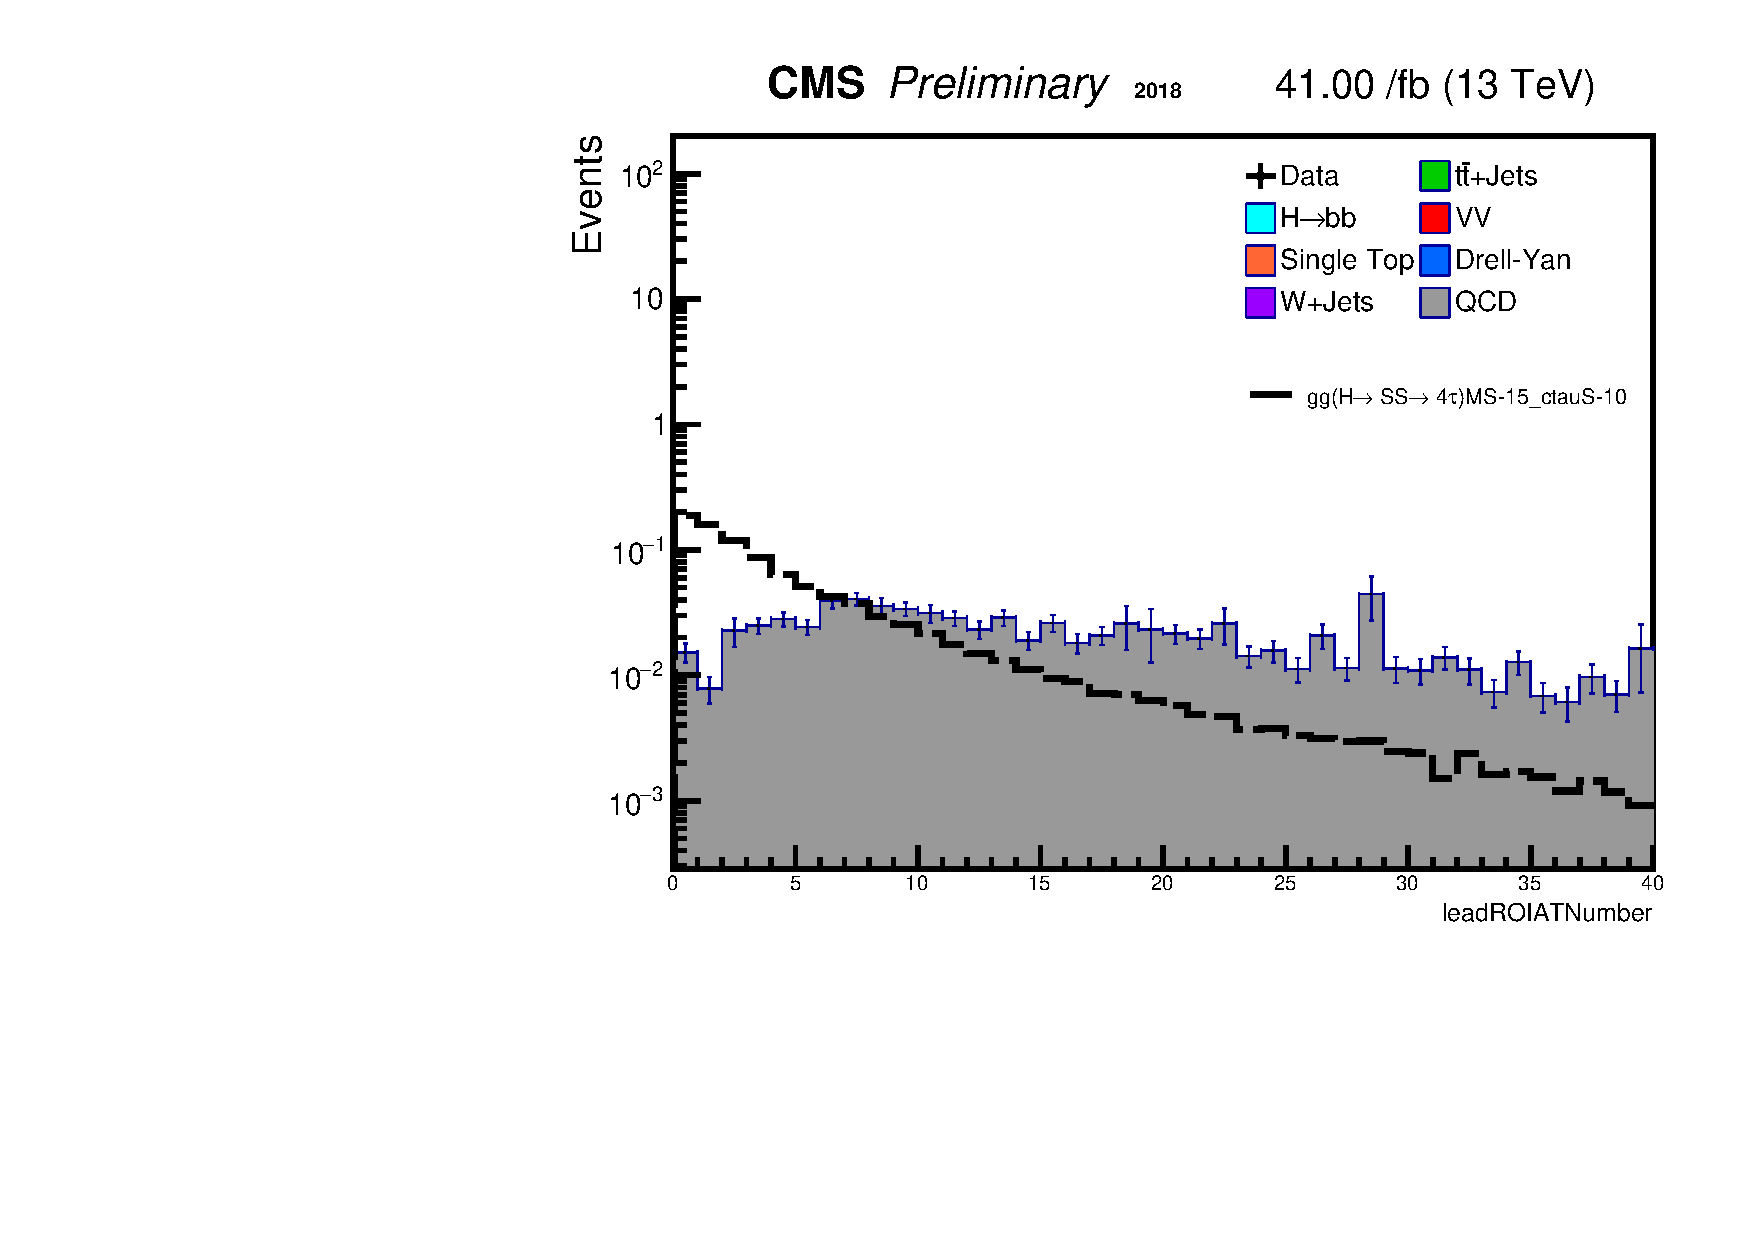
\includegraphics[width=0.47\linewidth]{figs/AnalysisNoteplot_MS-15_ctauS-10_leadROIATNumber.pdf}
%   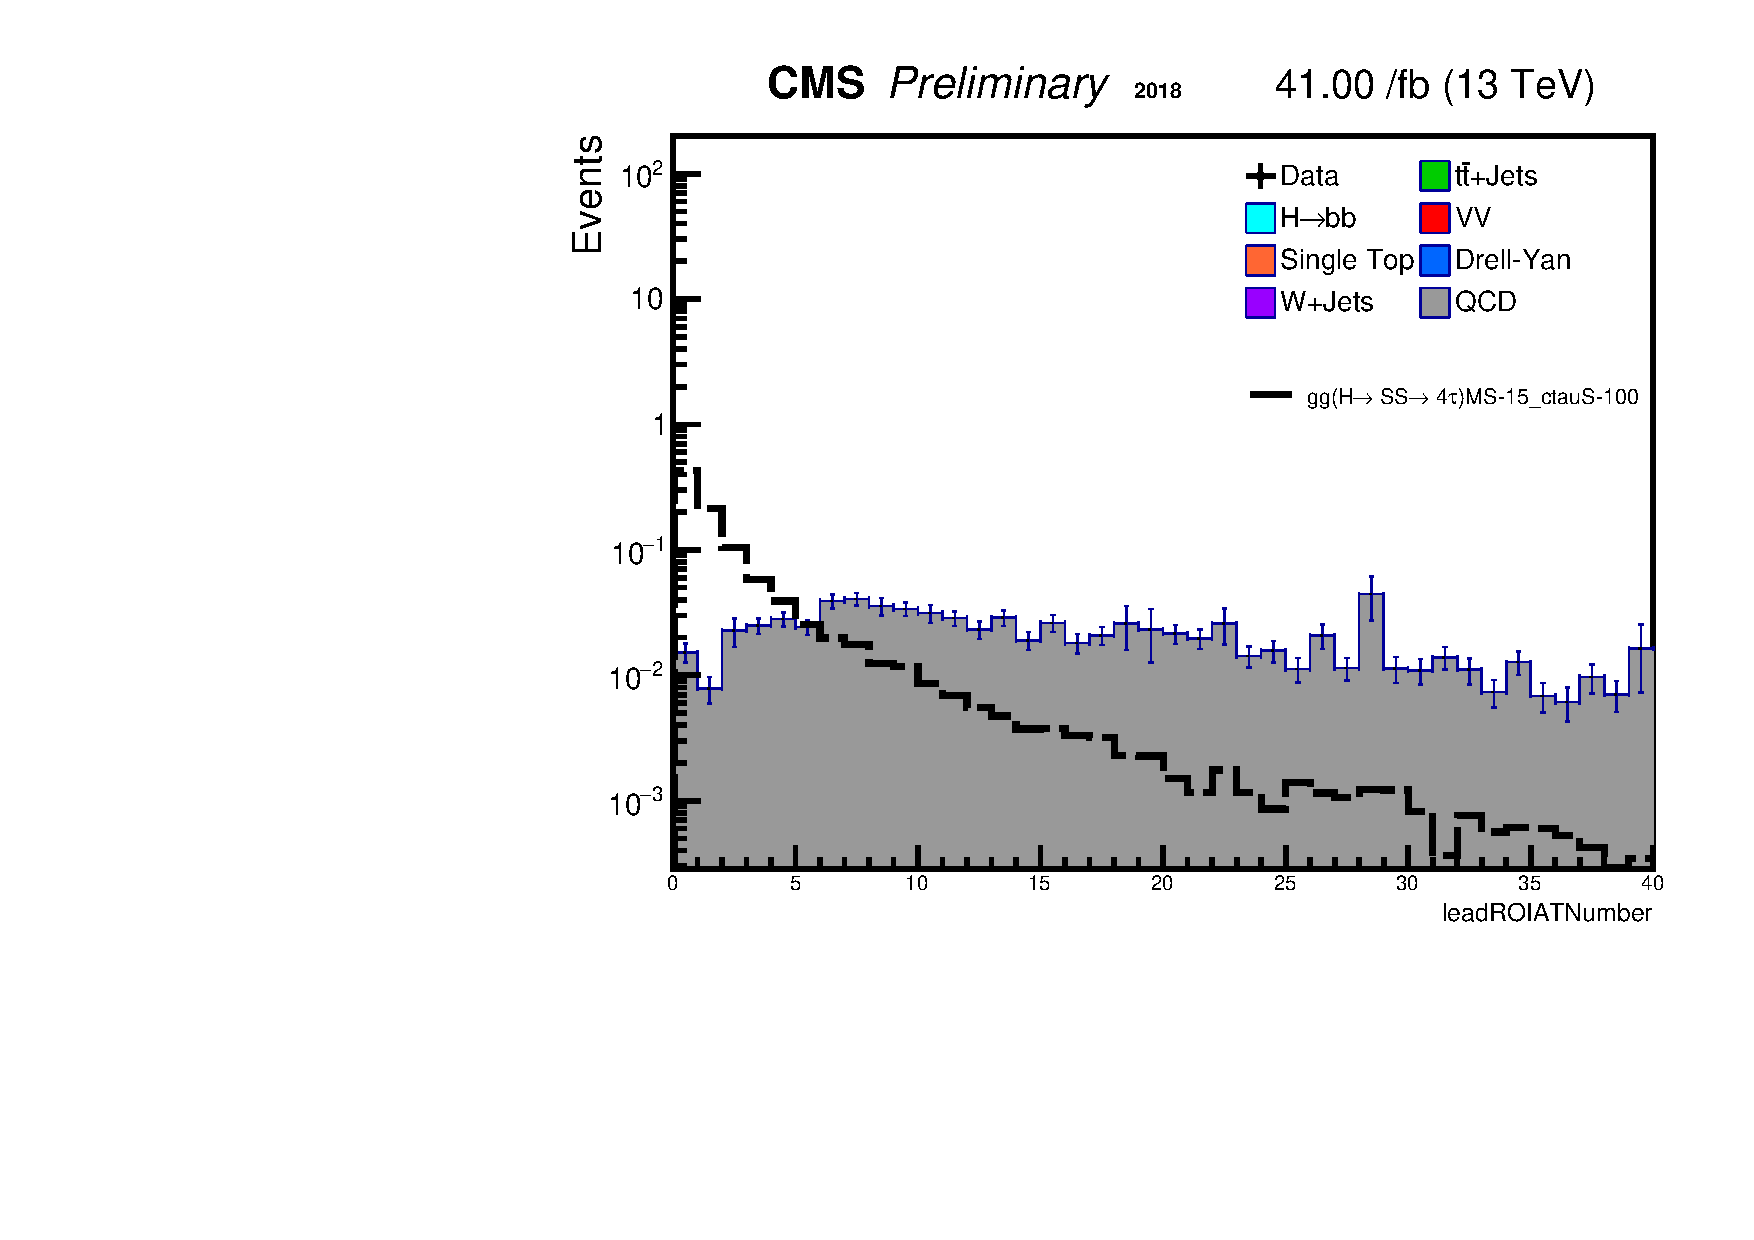
\includegraphics[width=0.47\linewidth]{figs/AnalysisNoteplot_MS-15_ctauS-100_leadROIATNumber.pdf}
% \end{figure}


%\section{Number of Annulus Tracks Associated with ROI}\label{ref:NumAnnulus}
% The tensorflow used for this analysis is trained with $p_T, \eta, \chi^{2}$, and other information of the annulus tracks (tracks that are inside ROI radius, but not fitted to vertex).
%Meanwhile, an ROI's total number of annulus tracks is not a direct input for ML and tensorflow can only learn such information indirectly via annulus tracks' $p_T$.
%Although having selected ROIs with high scores ($>$0.999), signal processes ROIs' number of annulus tracks show a quite different distribution from the background process.
%%Figure ~\ref{fig:ANnum}
%signal's high-scoring ROIs are mostly from the the exotic LLP scalar's decay into $\tau$ leptons. 
%%The $\tau$ leptons have most 3 charged tracks for 12\%, and 1 charged track for 80\% of its decay mode ~\cite{willbedonelater}
%Since the signal's high-score ROIs' are very well isolated, the ROI's number of annulus tracks is very low.
%QCD background events, which are our dominant background, have a poor isolation quality.
%Since QCD's high-scoring ROI's are poorly isolated due to QCD nature, these ROIs' numbers of annulus tracks are higher than the signal.
%More precisely, QCD's high-scoring ROI's are usually from B-mesons, which have higher track multiplicity than $\tau$ leptons.
%
%
%%% \begin{figure}[h!]
% \begin{figure}[h!]
%   \caption{Number of tracks in the annulus cone of the leading ROI. Left plot is for MS-15\_ctauS-10mm point, whereas the right plot is for MS-15\_cauS-100mm point}
%   \label{fig:ANleadSize}
%   \centering
%   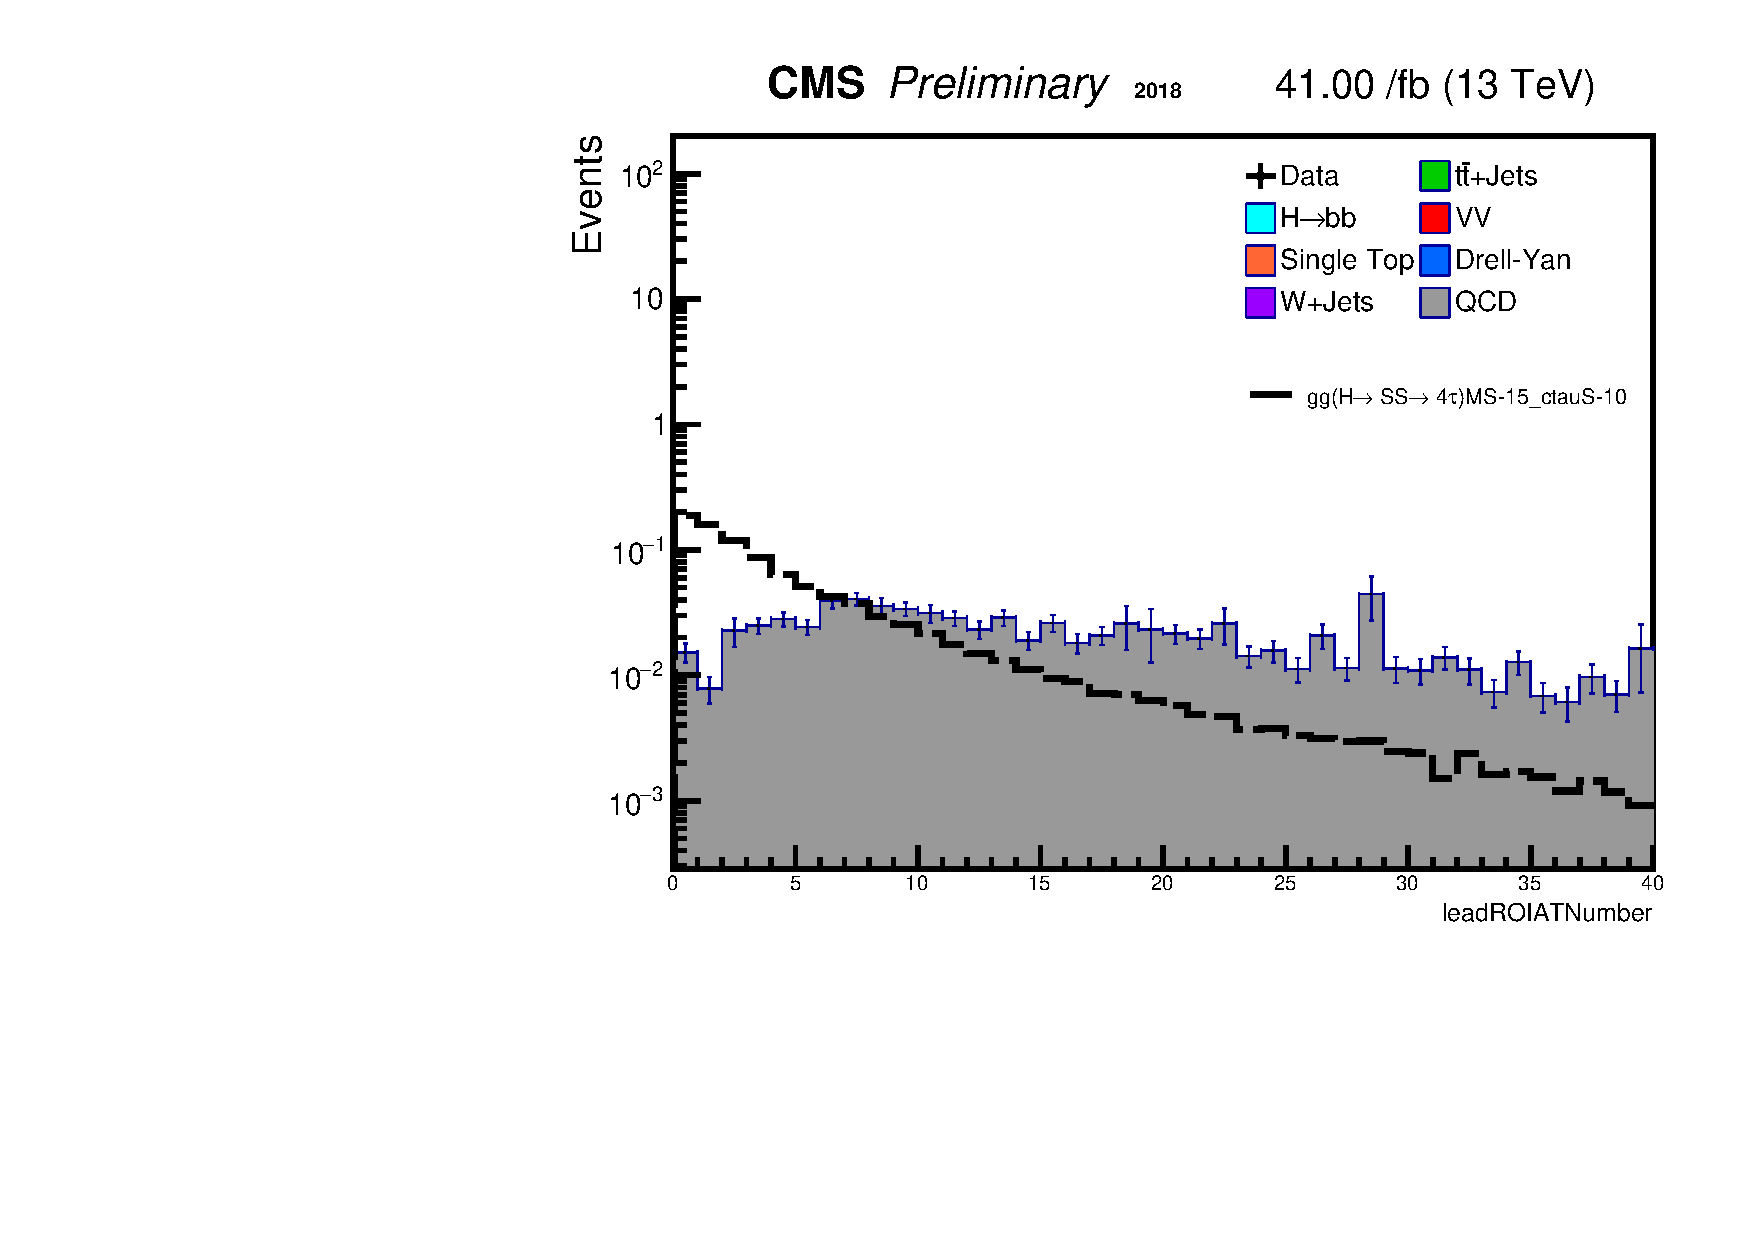
\includegraphics[width=0.47\linewidth]{figs/AnalysisNoteplot_MS-15_ctauS-10_leadROIATNumber.pdf}
%   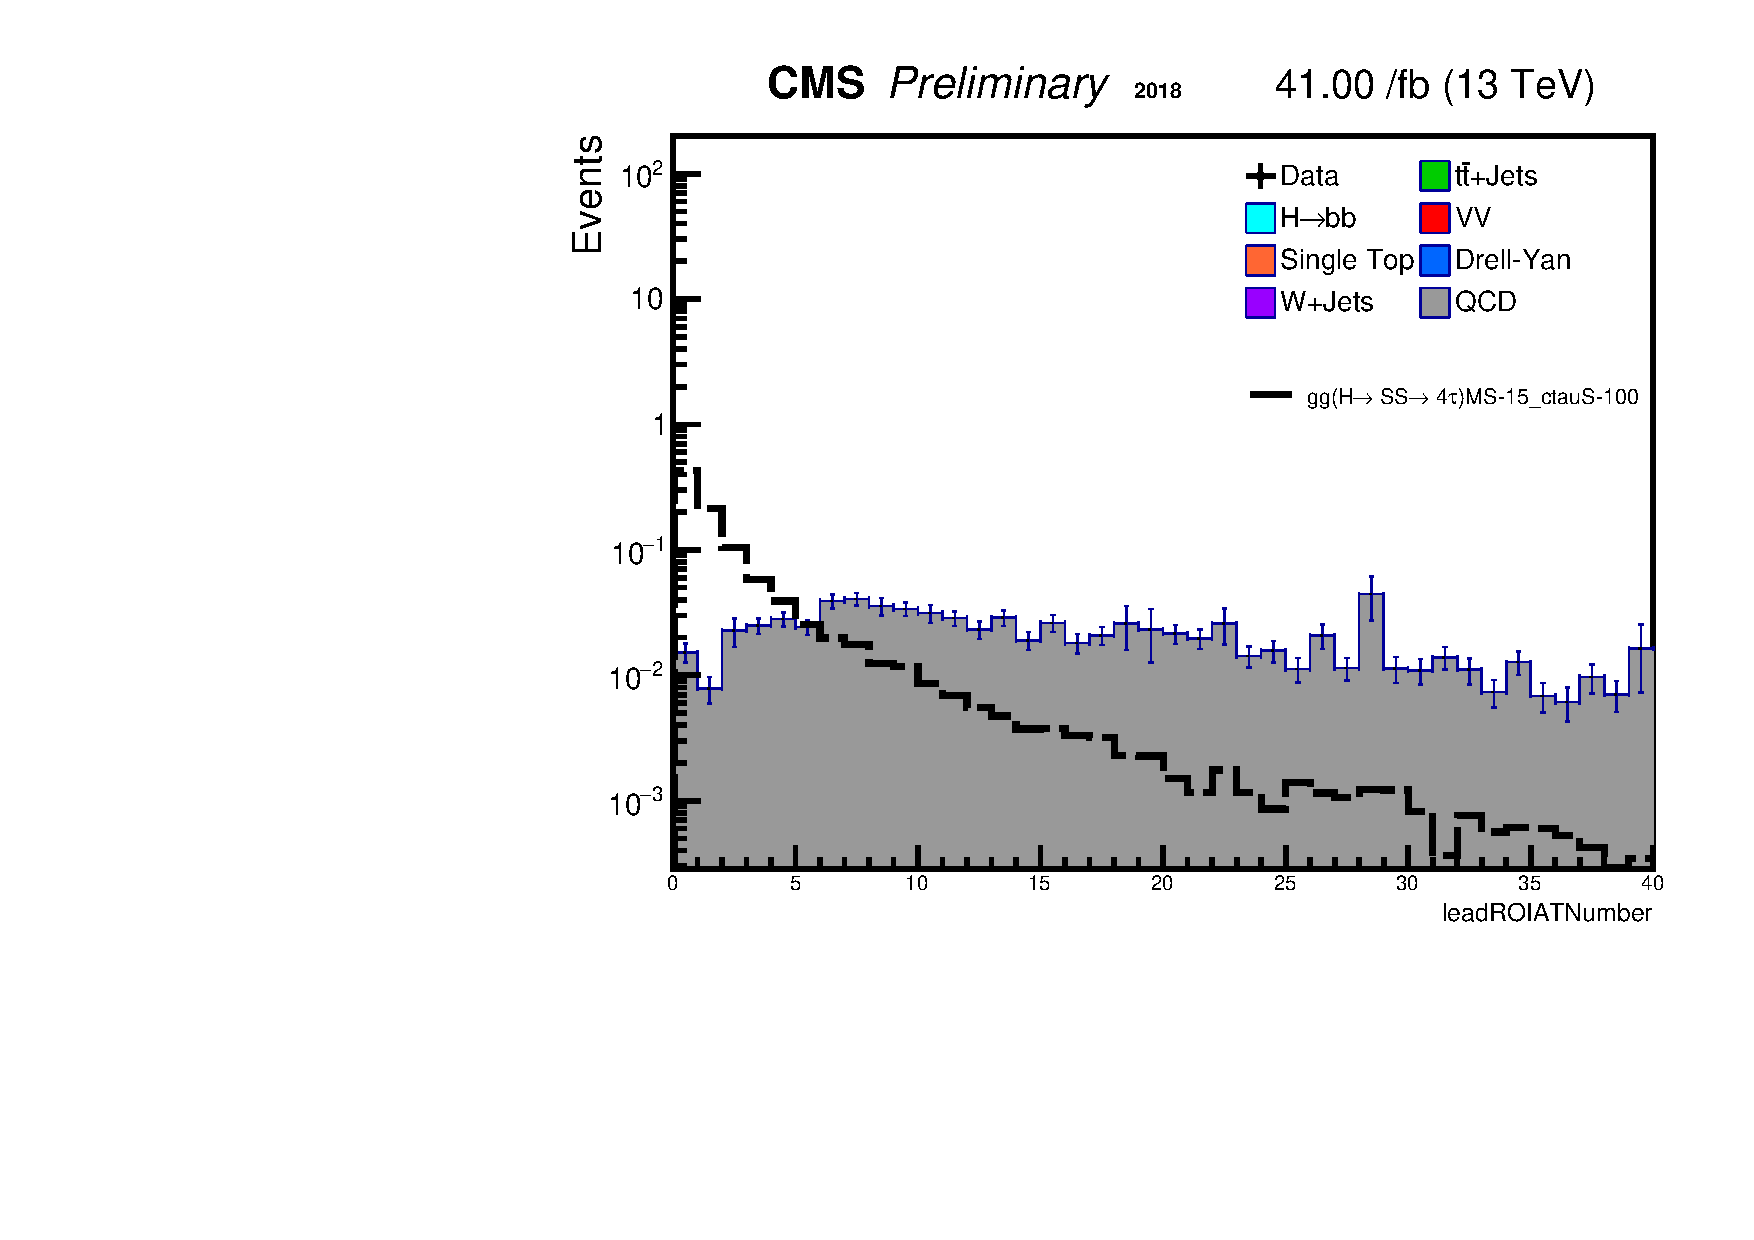
\includegraphics[width=0.47\linewidth]{figs/AnalysisNoteplot_MS-15_ctauS-100_leadROIATNumber.pdf}
% \end{figure}
%
%
%
